\section{Observaciones y Resultados}
\vs{-30}
% colspec={|X[j,h]|c|c|}  <--- Versión anterior (3 columnas)
\begin{longtblr}[]{colspec={|X[c,m]|X[c,m]|}, hlines}
    \SetCell[c=2]{j}{\textbf{Observación: Prueba 01}}  \\
    {En las siguientes gráficas se utilizó el modelo sm (predeterminado por el simulador). La primer gráfica muestra la masa invariante $m(\mu^{+}\mu^{-})$, mientras que la segunda gráfica está en escala logarítmica para el eje y. Los datos de la masa empiezan a partir de los $20\,[GeV]$, lo cual se debe a las condiciones que imponen la \textit{run\_card.dat} y posiblemente \textit{delphes\_card.dat}.} & {\textit{Proximas metas}: Lograr datos con masas $m_{\mu\mu}<20.0\,[GeV]$ y motivos del porque se tiene una masa para $\mu^{-}=0$.} \\
    \SetCell[c=2]{c}{\textbf{Modelo sm}} \\
    {\textit{Escala lineal en ambos ejes}\\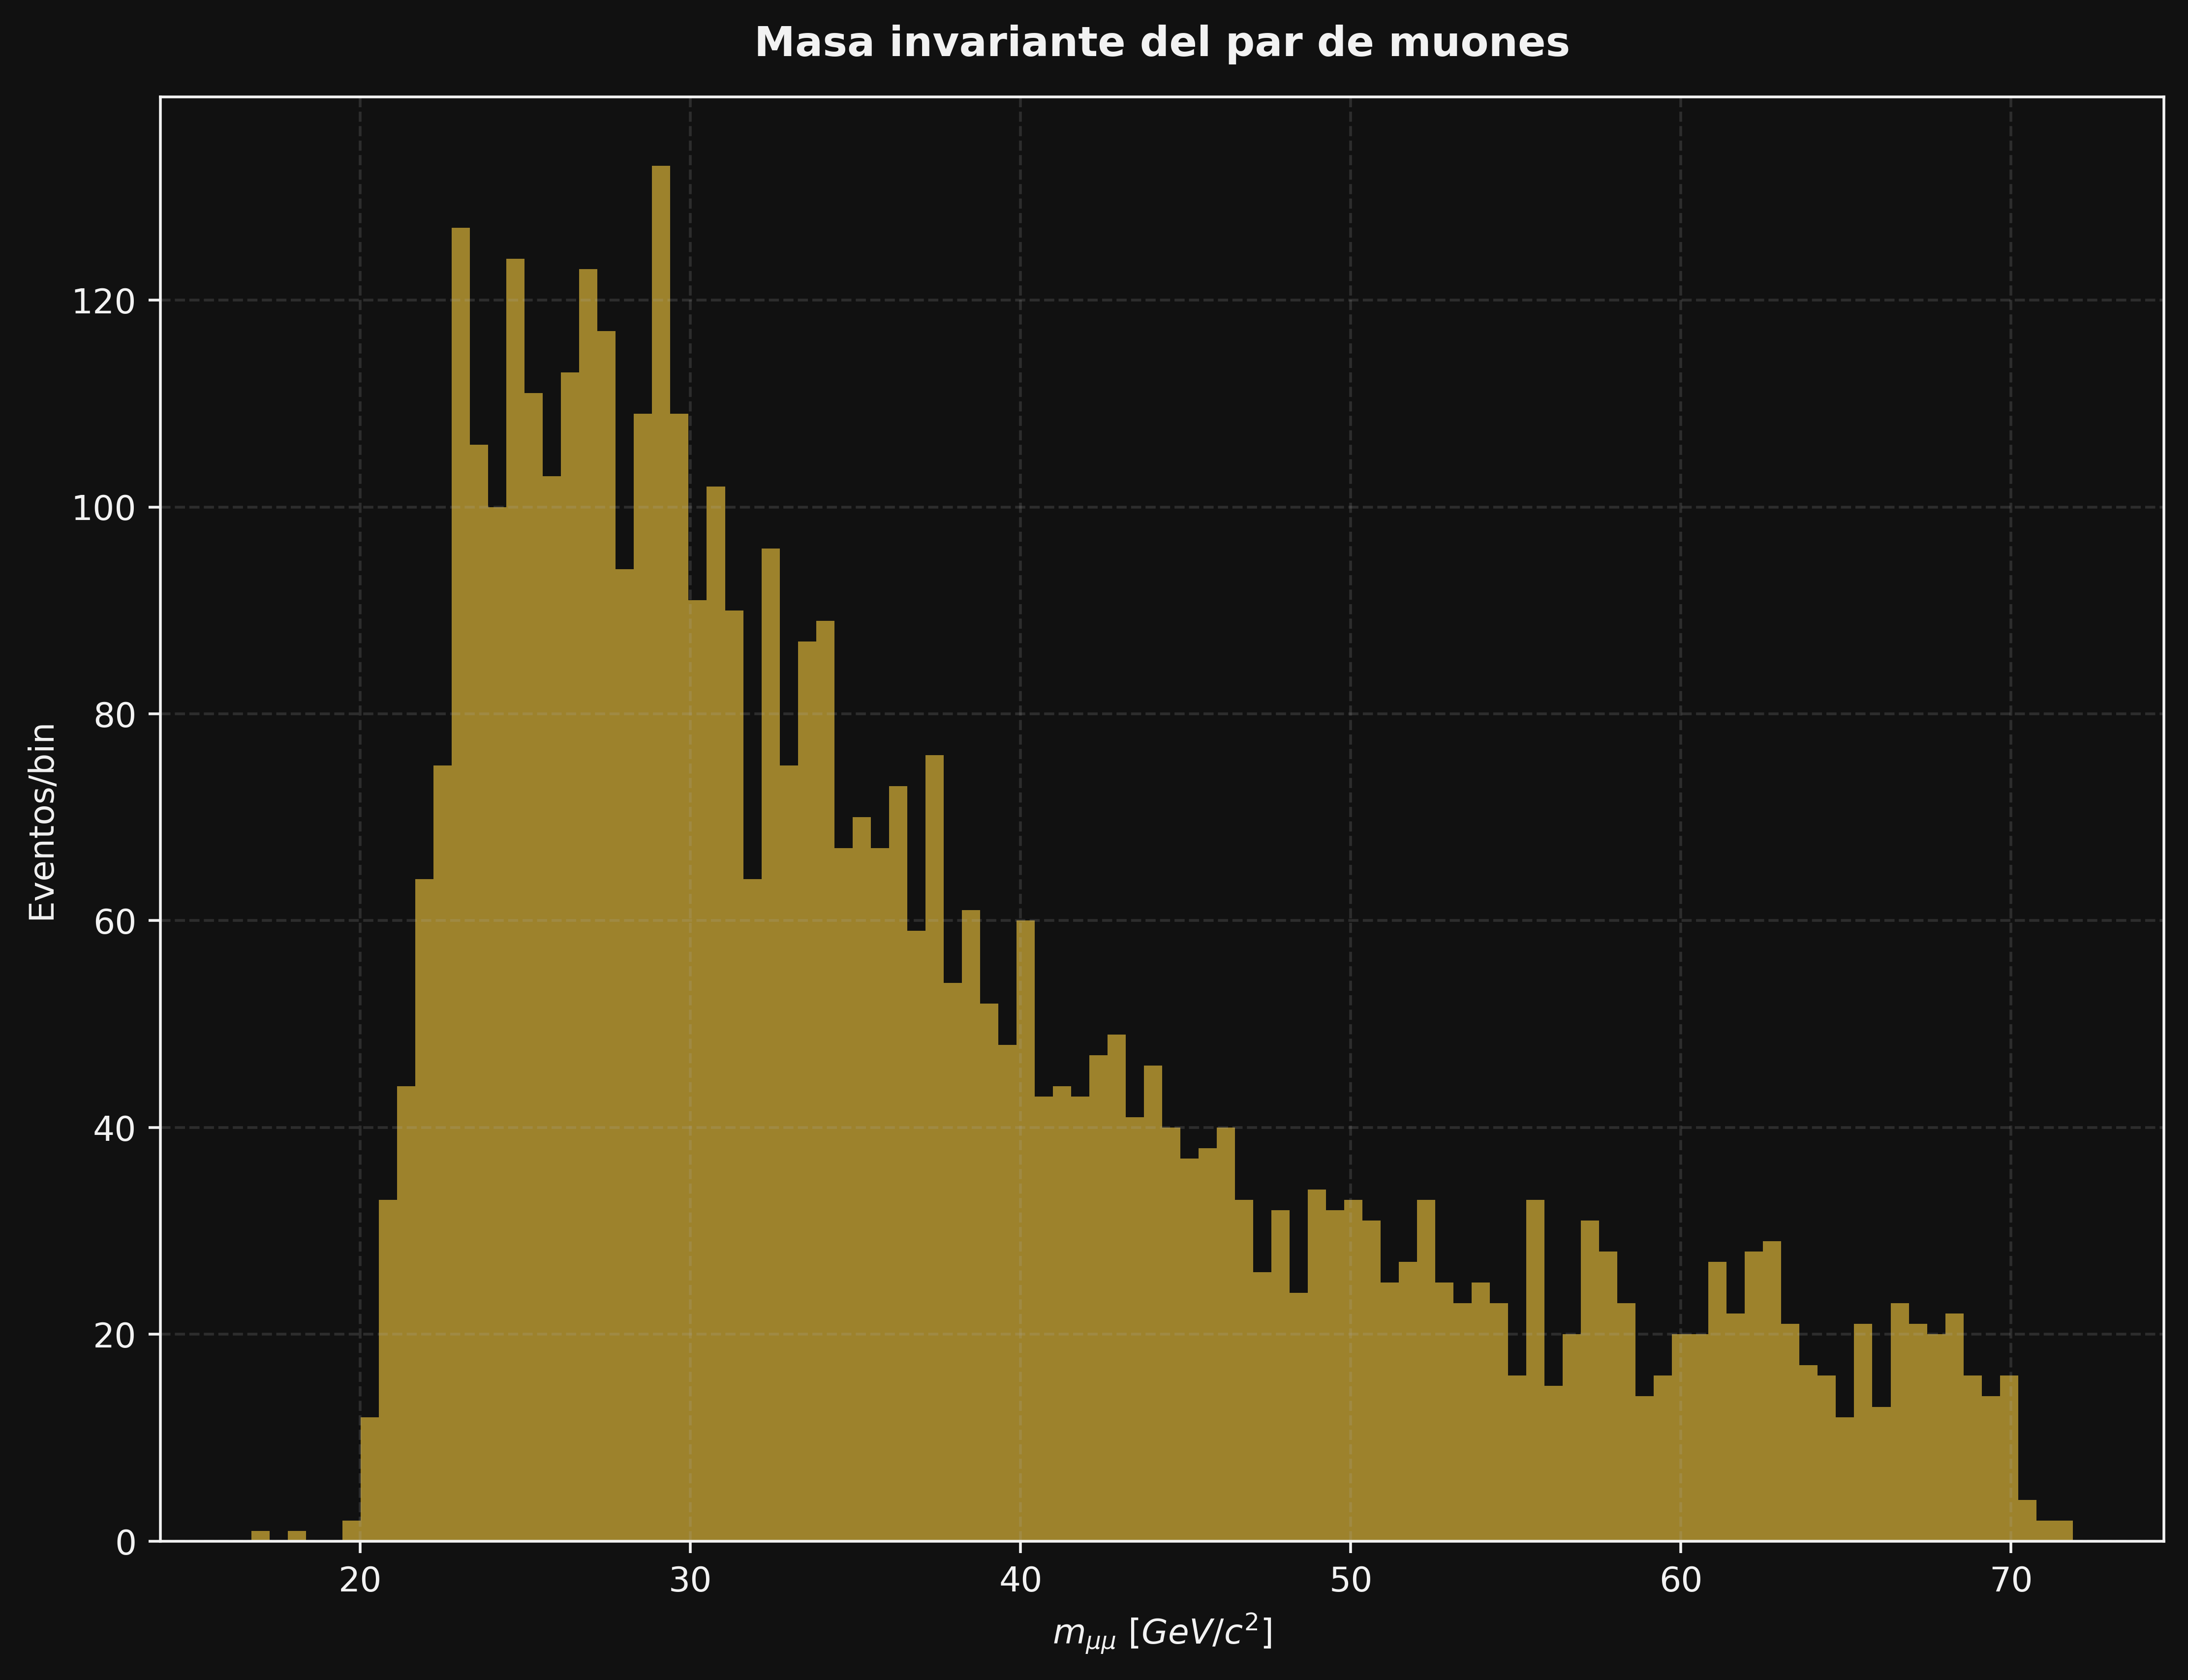
\includegraphics[width=\linewidth]{../assets/images/delphes/c00/two_muon_mass_01.png}} & {\textit{Escala logarítmica solamente en el eje y}\\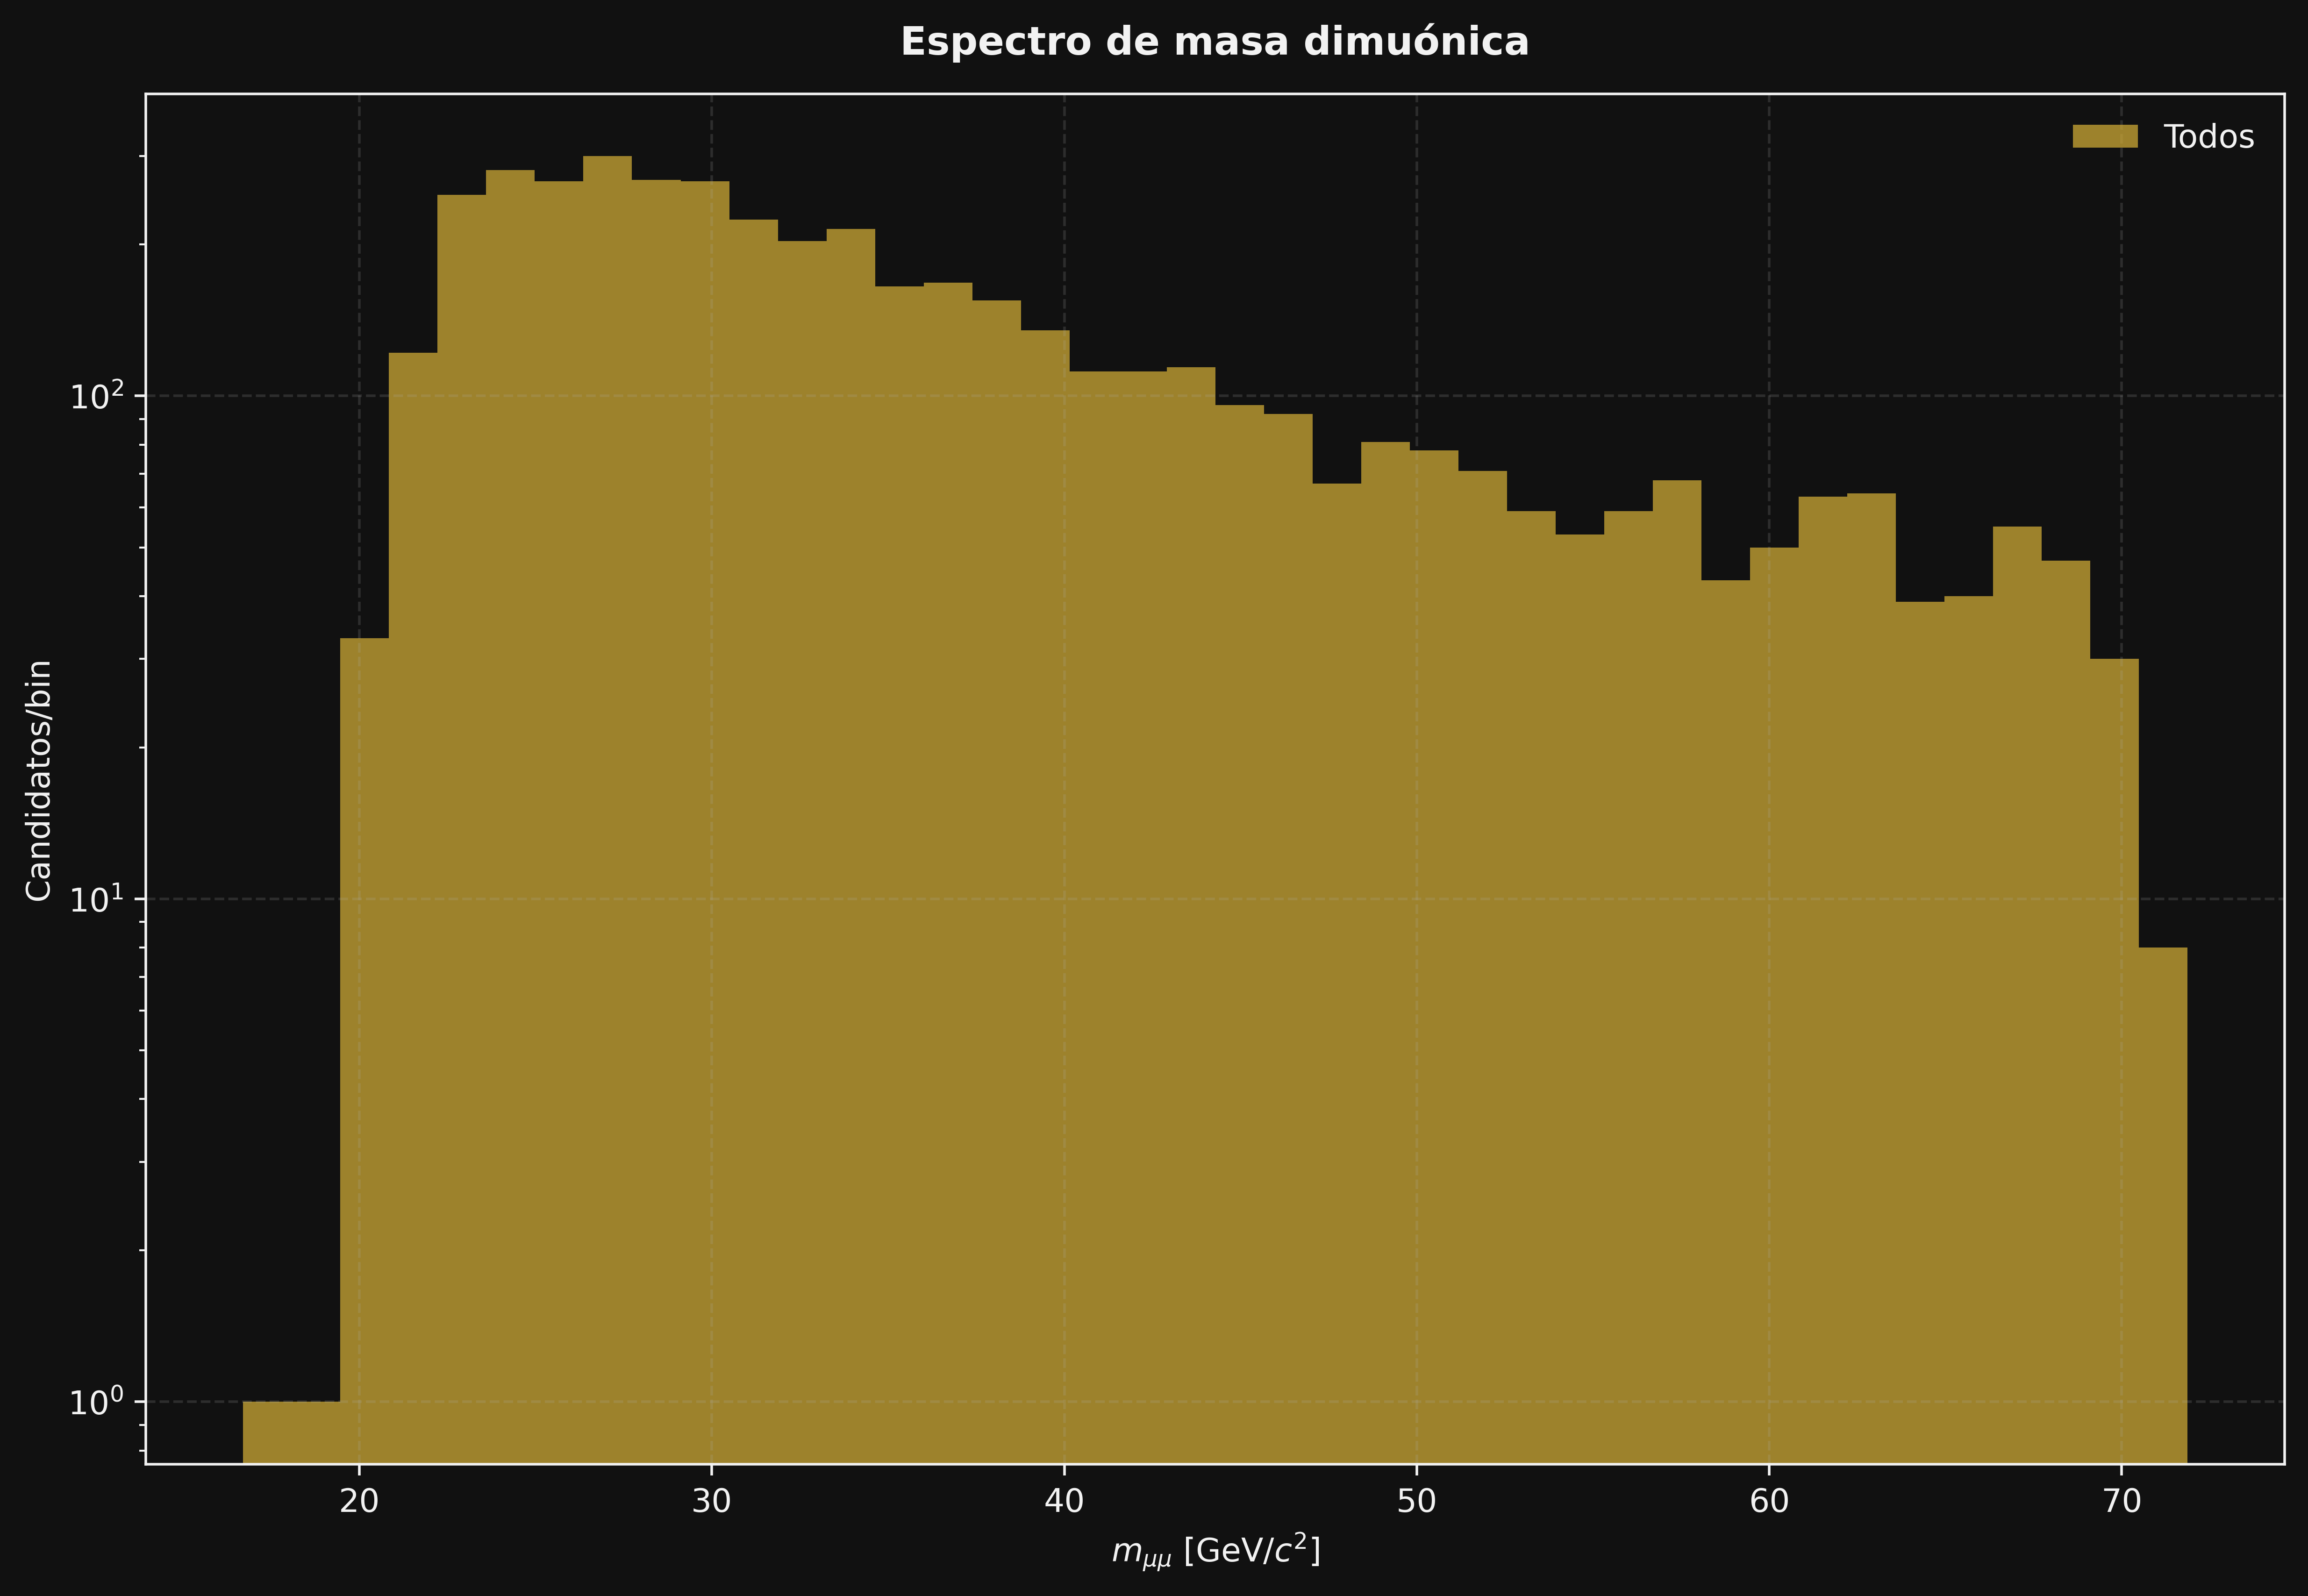
\includegraphics[width=\linewidth]{../assets/images/delphes/c00/dimuon_mass_01.png}} \\\hline\hline
    \SetCell[c=2]{j}{\textbf{Observación: Prueba 02}} \\
    {Modelos empleados sm y sm-full. Las primeras dos gráficas (de cada apartado) corresponden a un corte de mmll y mmnl de $10.0\,[GeV]$ (masa invariante), mientras que las últimas dos gráficas corresponden a un corte para masa invariante de $70.0\,[GeV]$ (con escala logarítmica los ejes x, y). Se aplicaron cortes para que la pseudo-rapidez ($\eta$) se encuentre dentro del rango de $2<\eta<5$ (para cumplir con el criterio del LHCb).} & {\textit{Proximas metas}: Buscar aceptaciones/parámetros del LHCb para la detección de muones.} \\
    \textbf{Modelo sm} & \textbf{Modelo sm-full} \\
    { \textit{X: esc. Lineal \& Y: esc. log. (sin corte) - 10 $[GeV]$}\\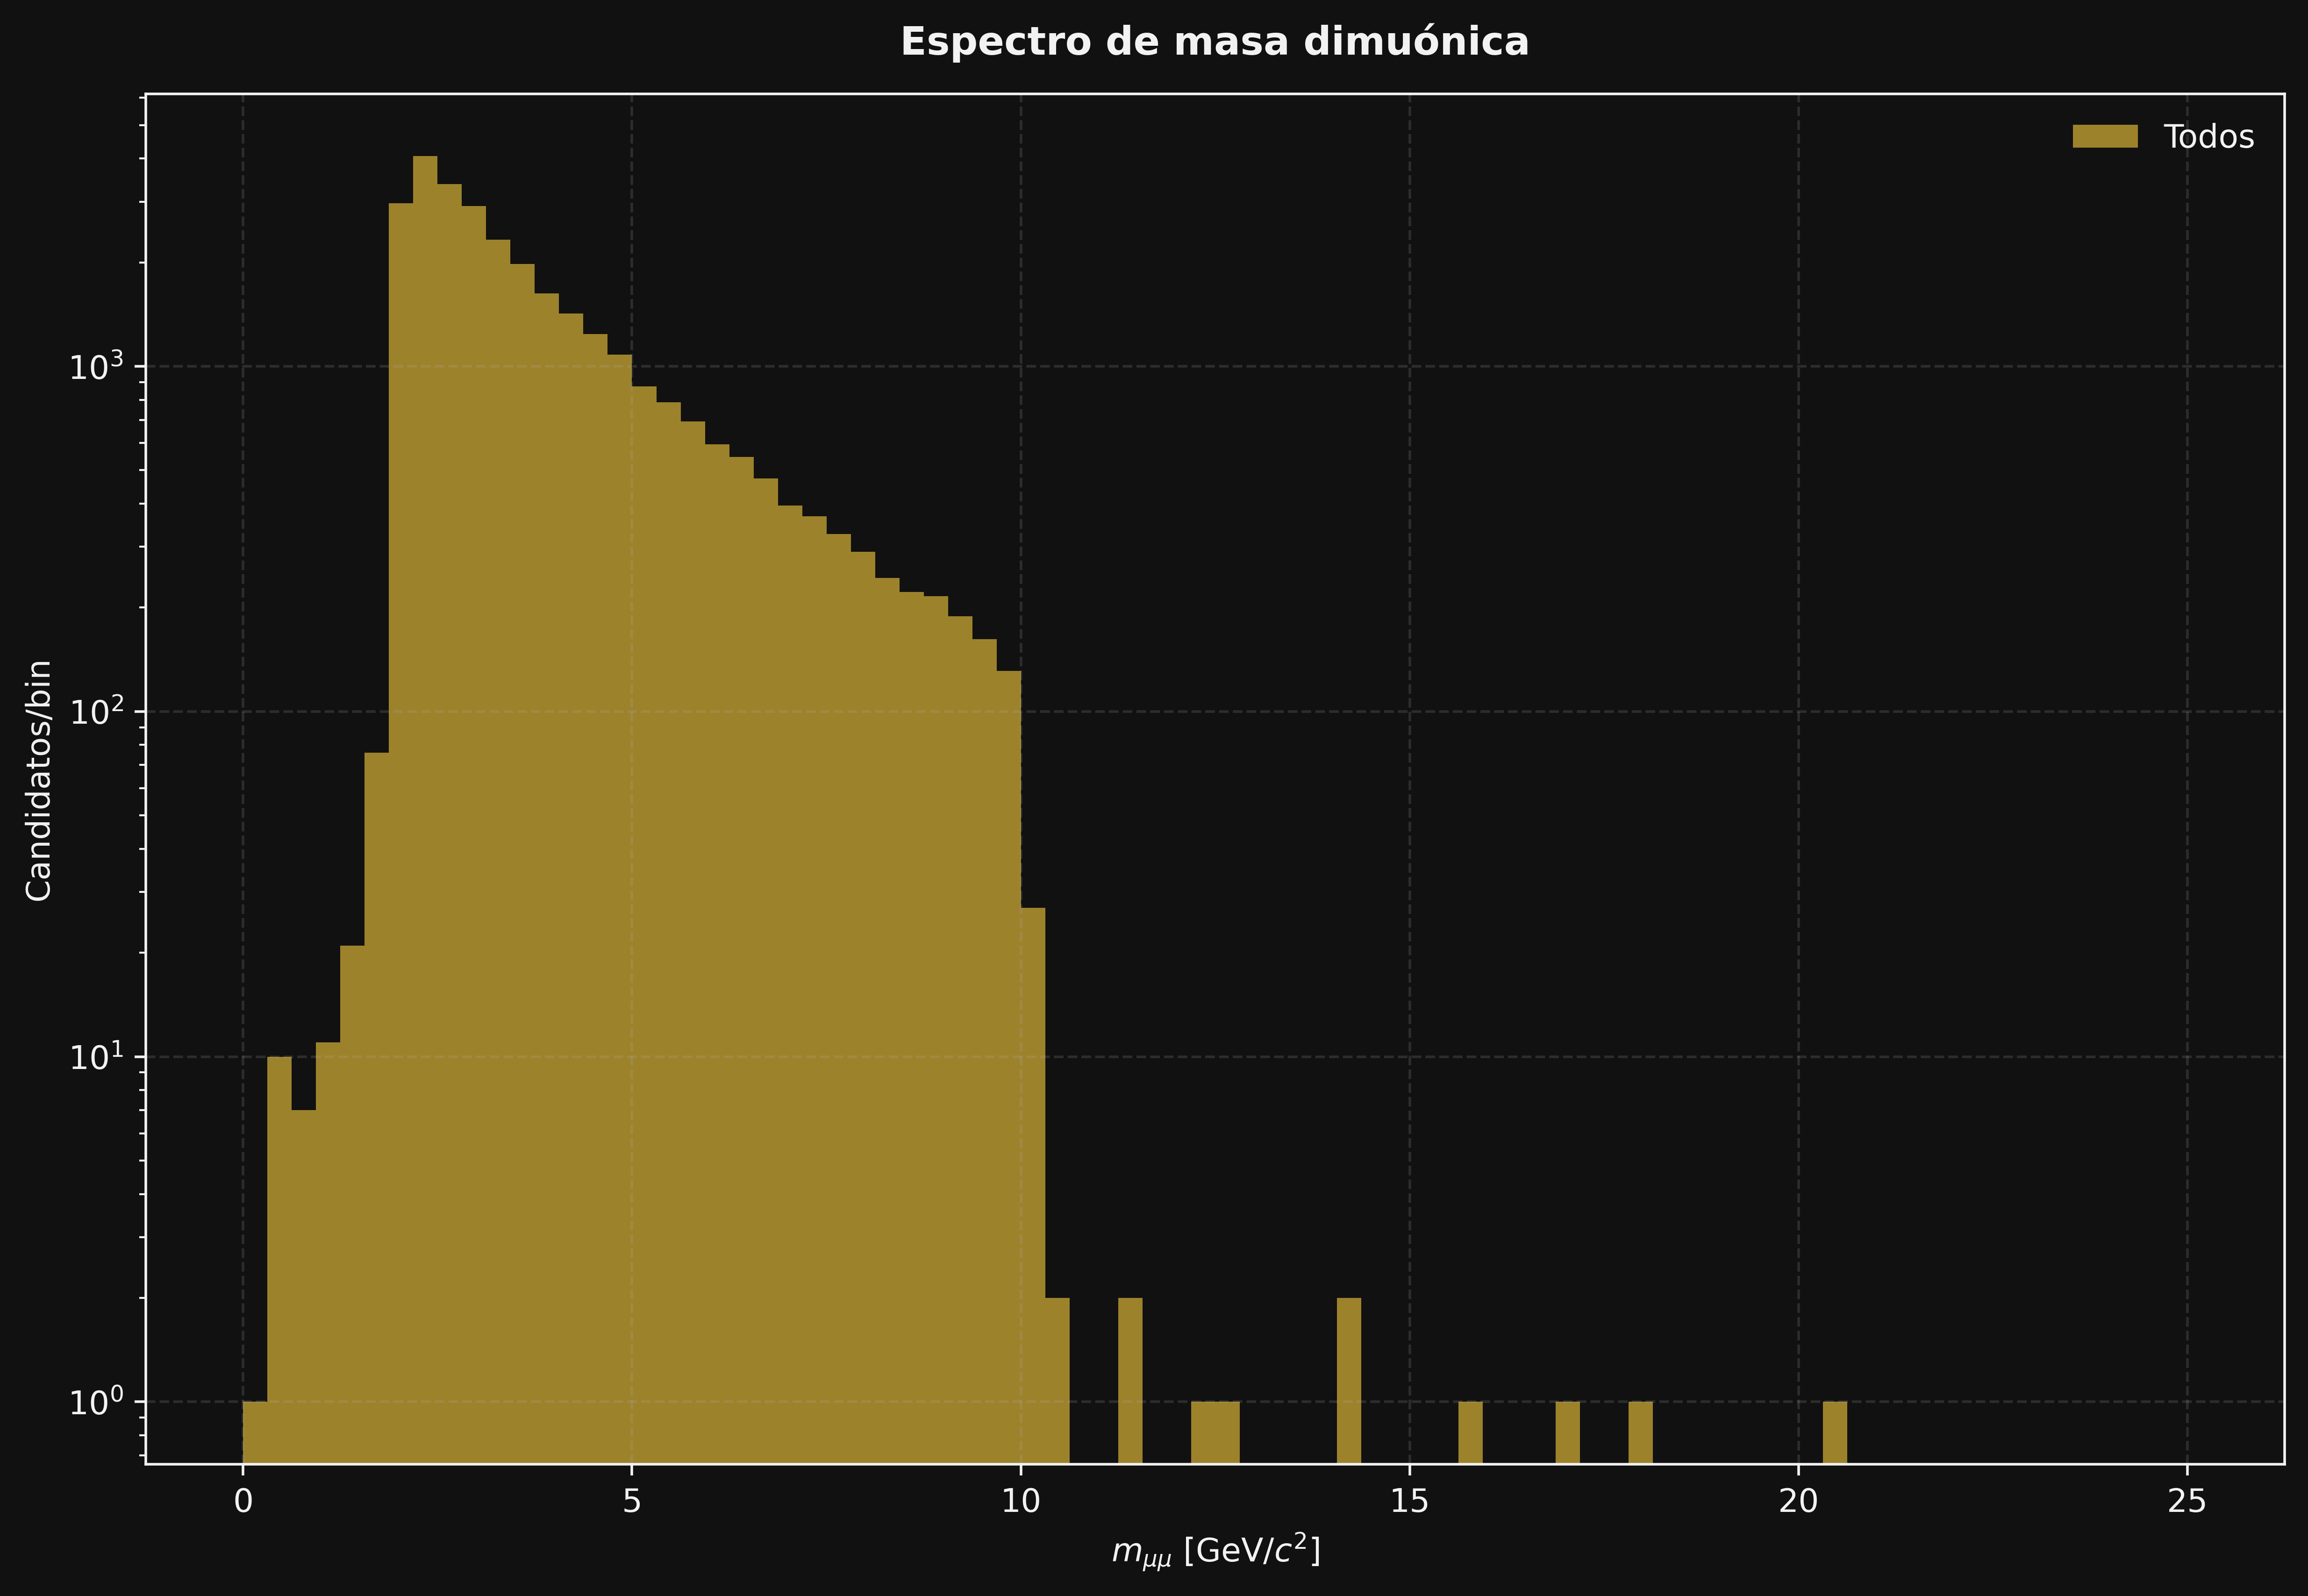
\includegraphics[width=\linewidth]{../assets/images/delphes/sm_model/c01/dimuon_mass_01.png} } & { \textit{X: esc. Lineal \& Y: esc. log. (sin corte) - 10 $[GeV]$}\\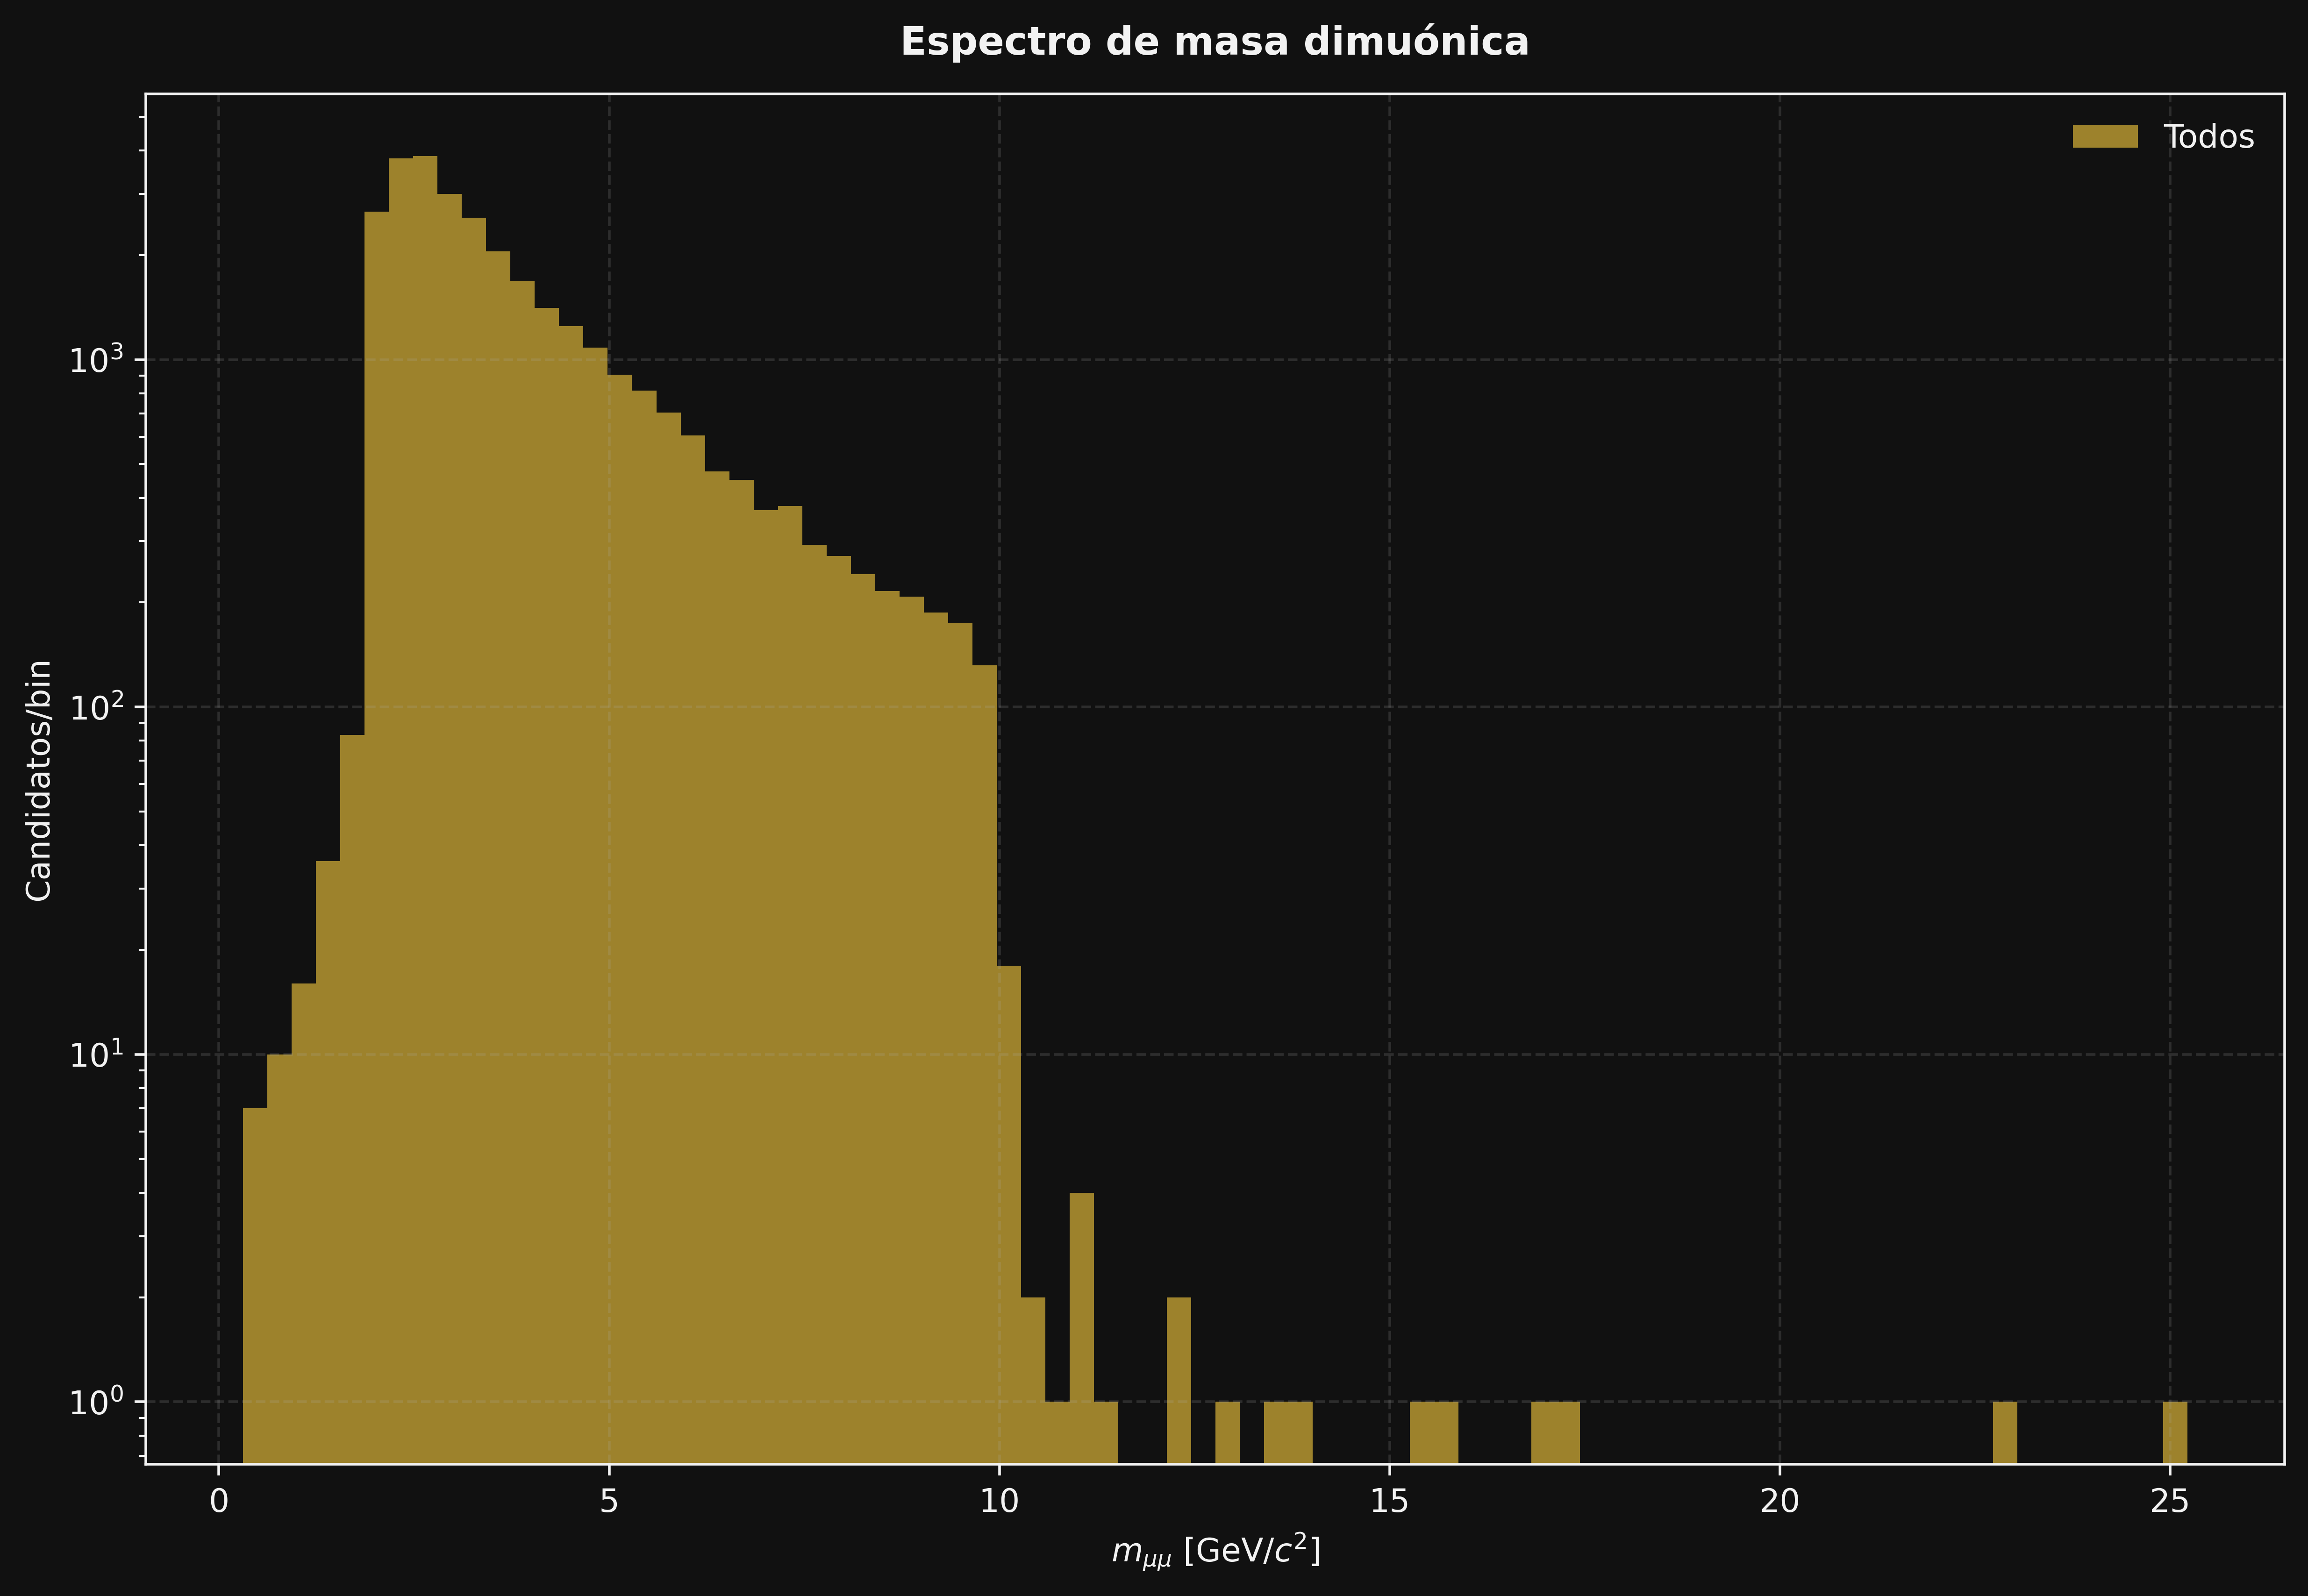
\includegraphics[width=\linewidth]{../assets/images/delphes/smf_model/c01/dimuon_mass_01.png} } \\
    { \textit{X: esc. Lineal \& Y: esc. log. (corte) - 10 $[GeV]$}\\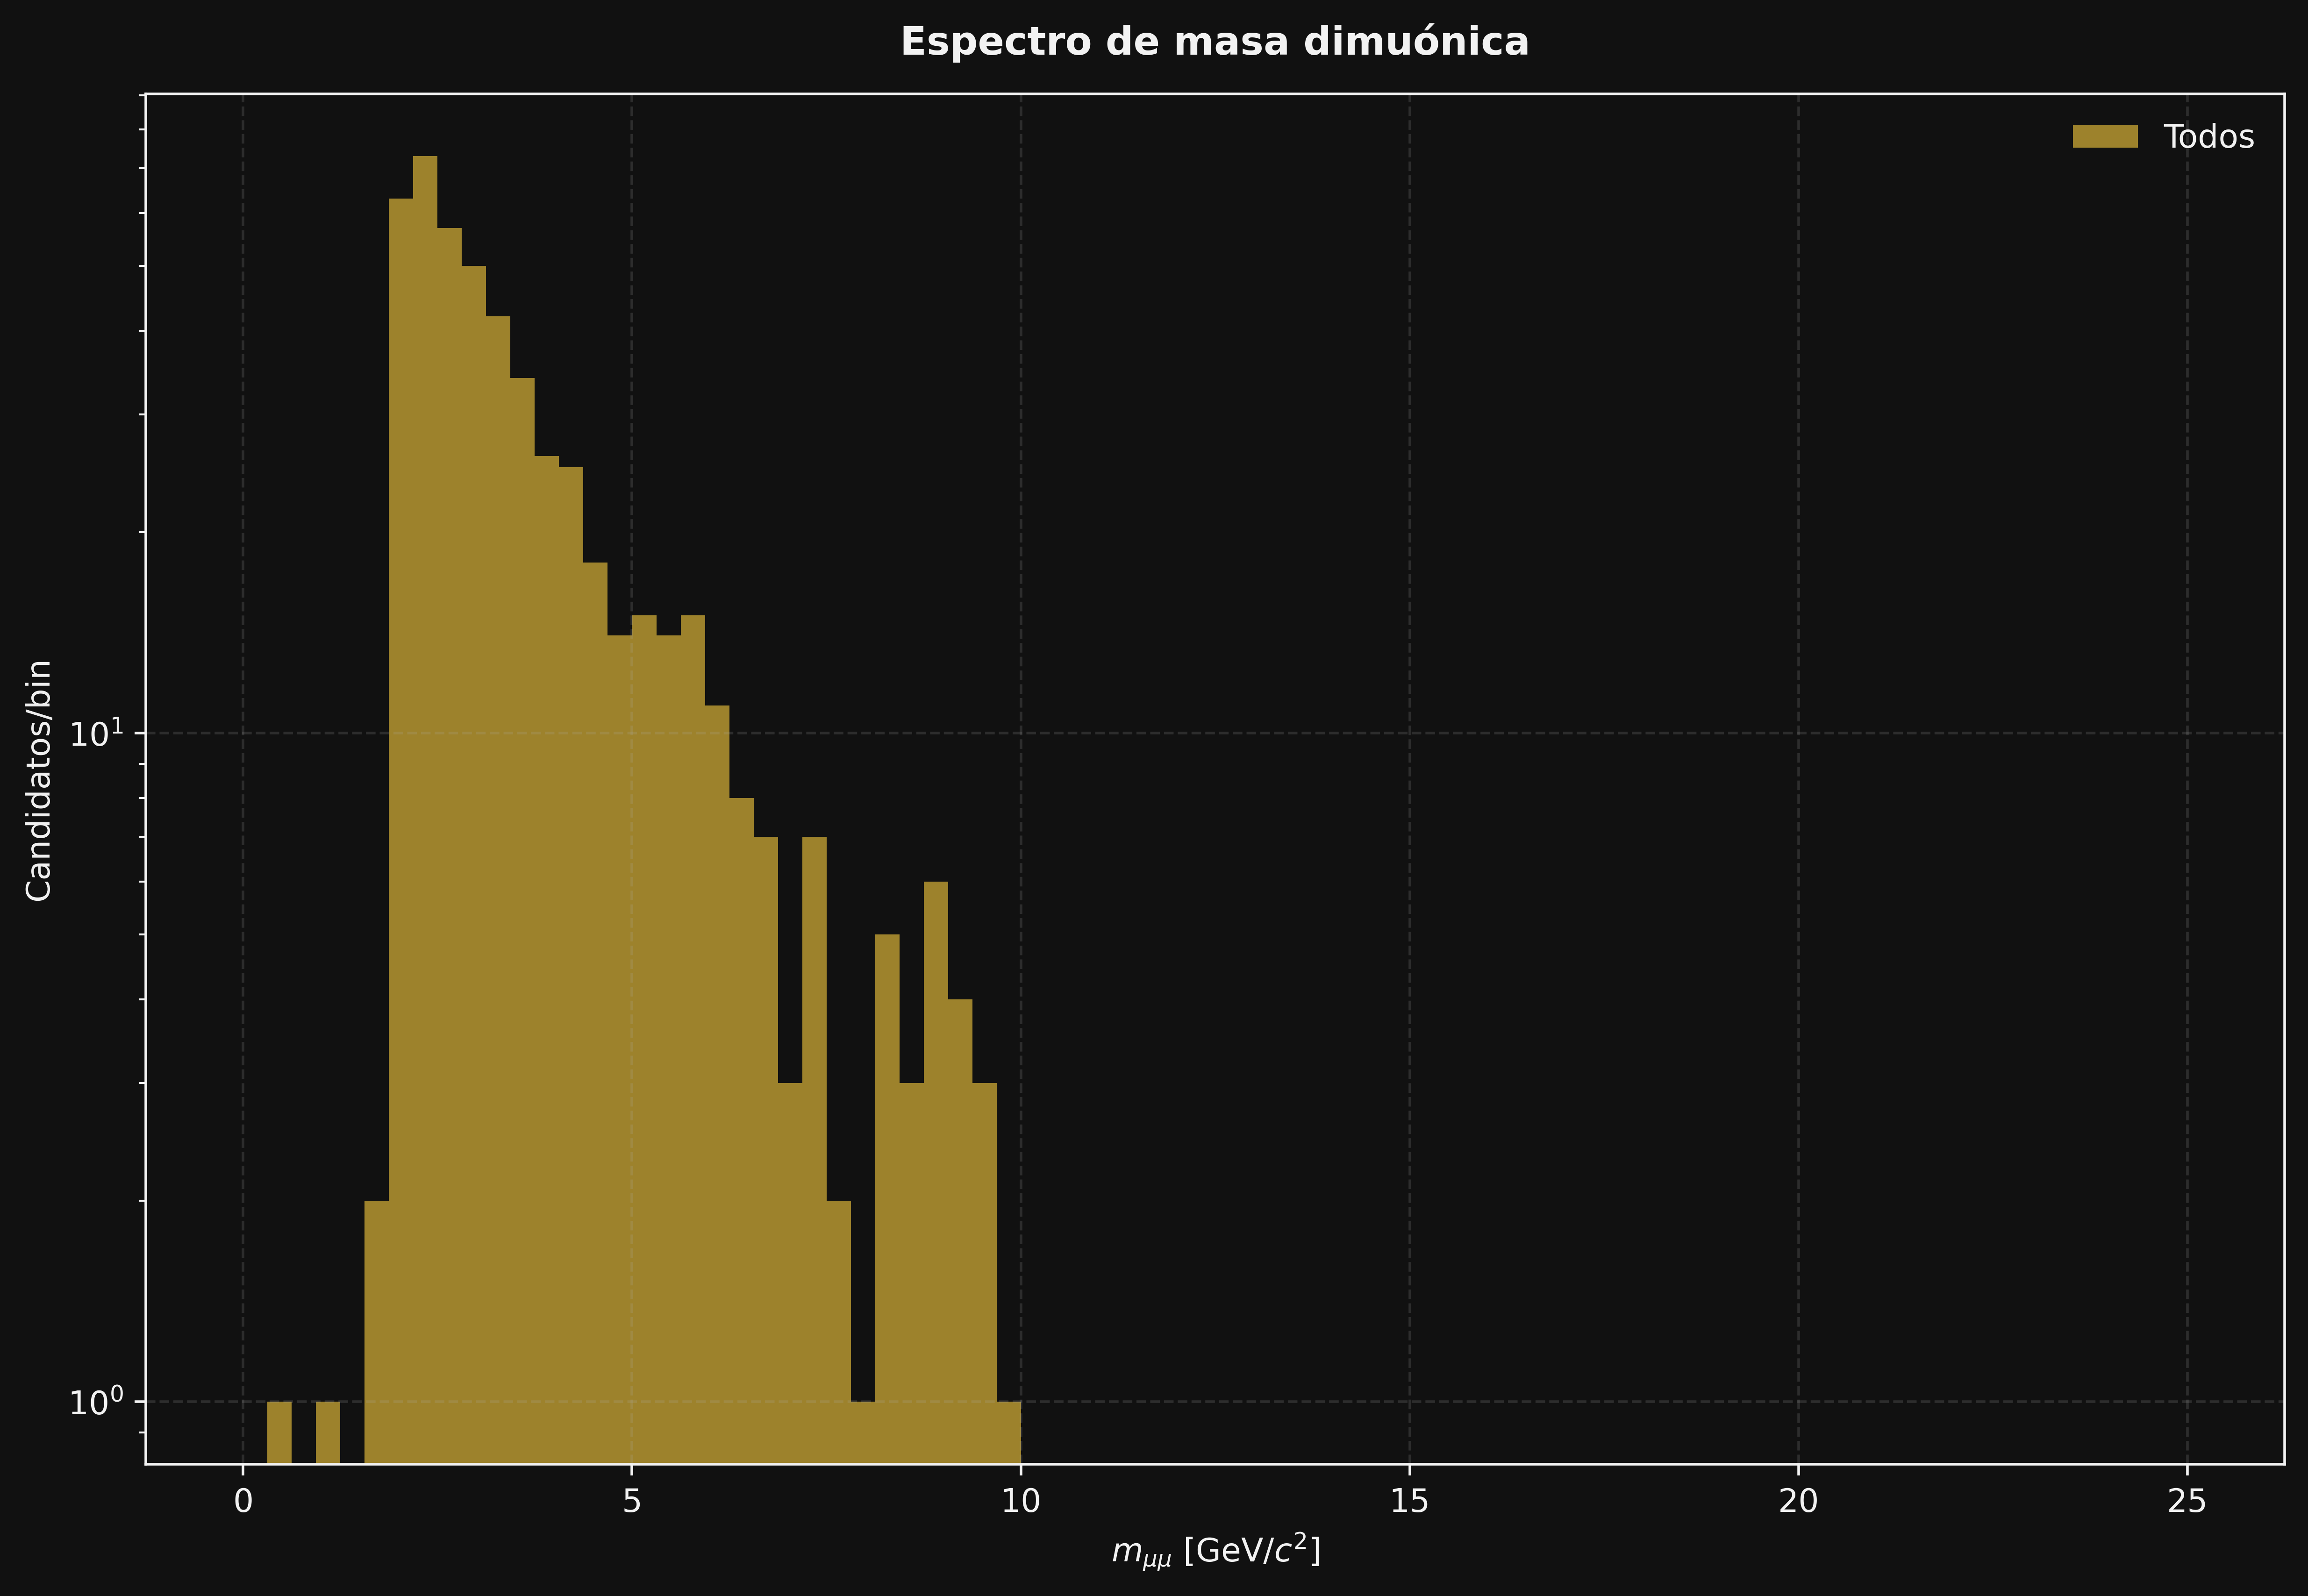
\includegraphics[width=\linewidth]{../assets/images/delphes/sm_model/c01/dimuon_mass_01_cut.png} } & { \textit{X: esc. Lineal \& Y: esc. log. (corte) - 10 $[GeV]$}\\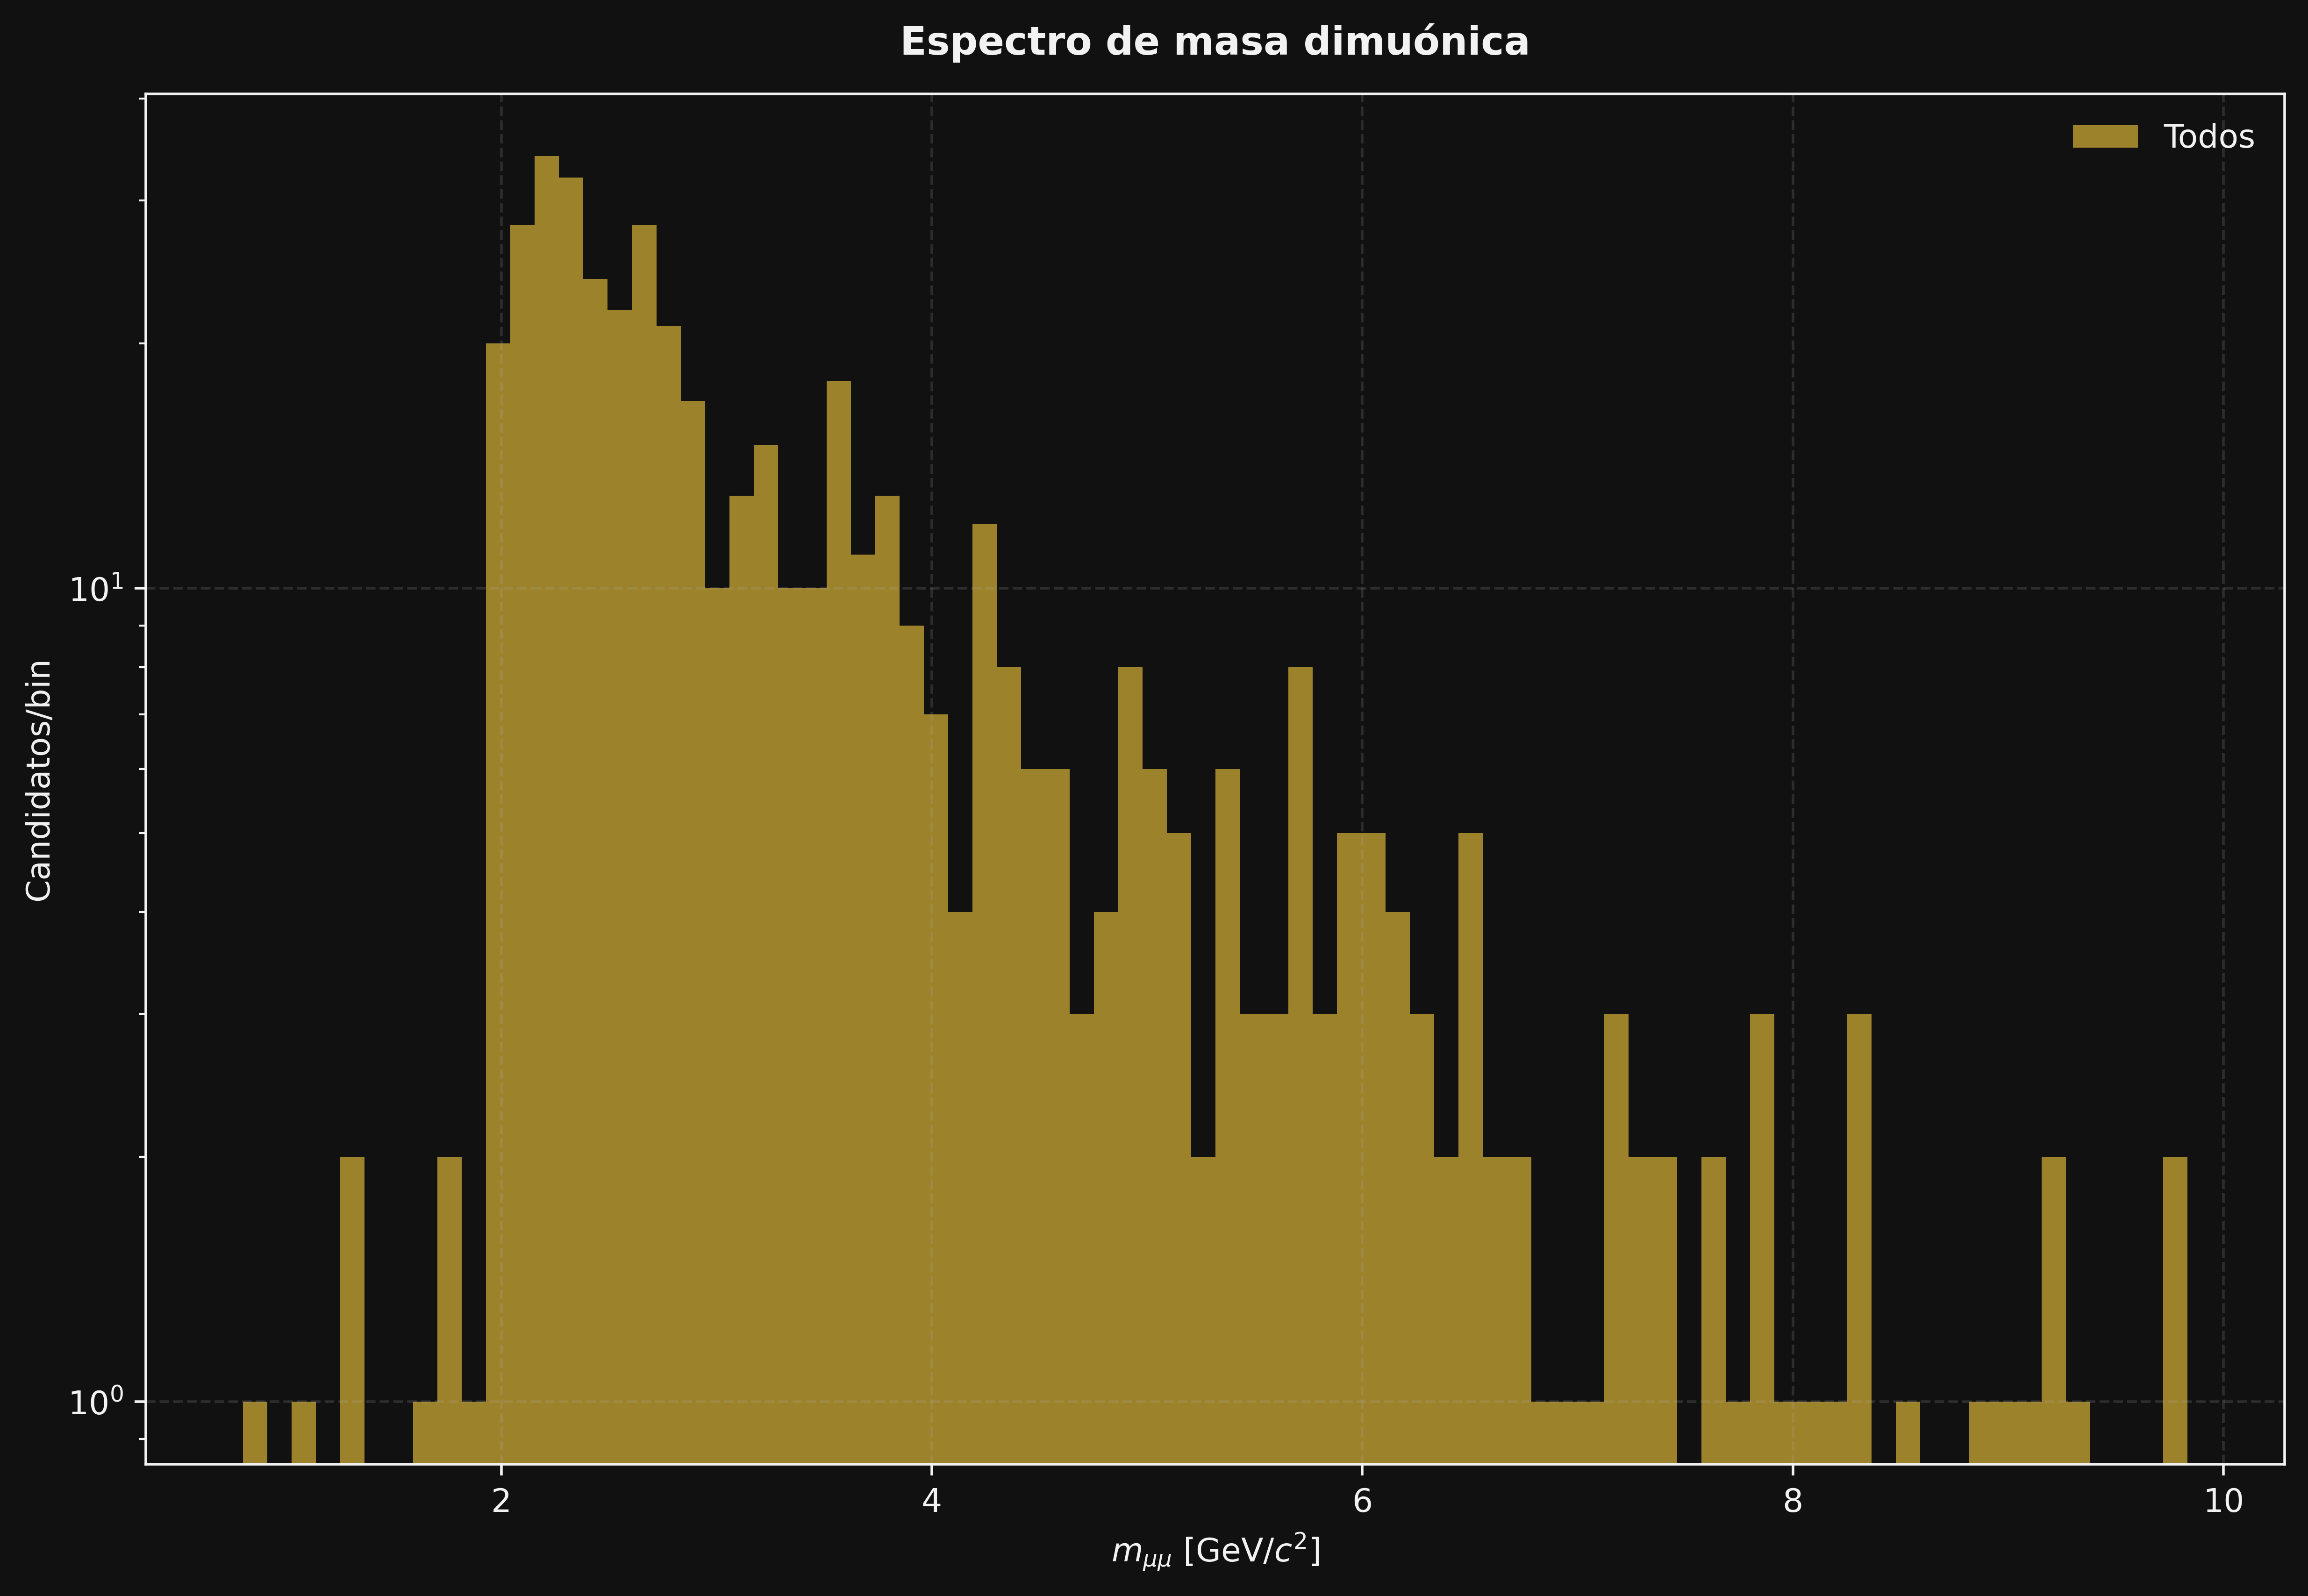
\includegraphics[width=\linewidth]{../assets/images/delphes/smf_model/c01/dimuon_mass_01_cut.png} } \\
    { \textit{X: esc. log. \& Y: esc. log. (sin corte) - 70 $[GeV]$}\\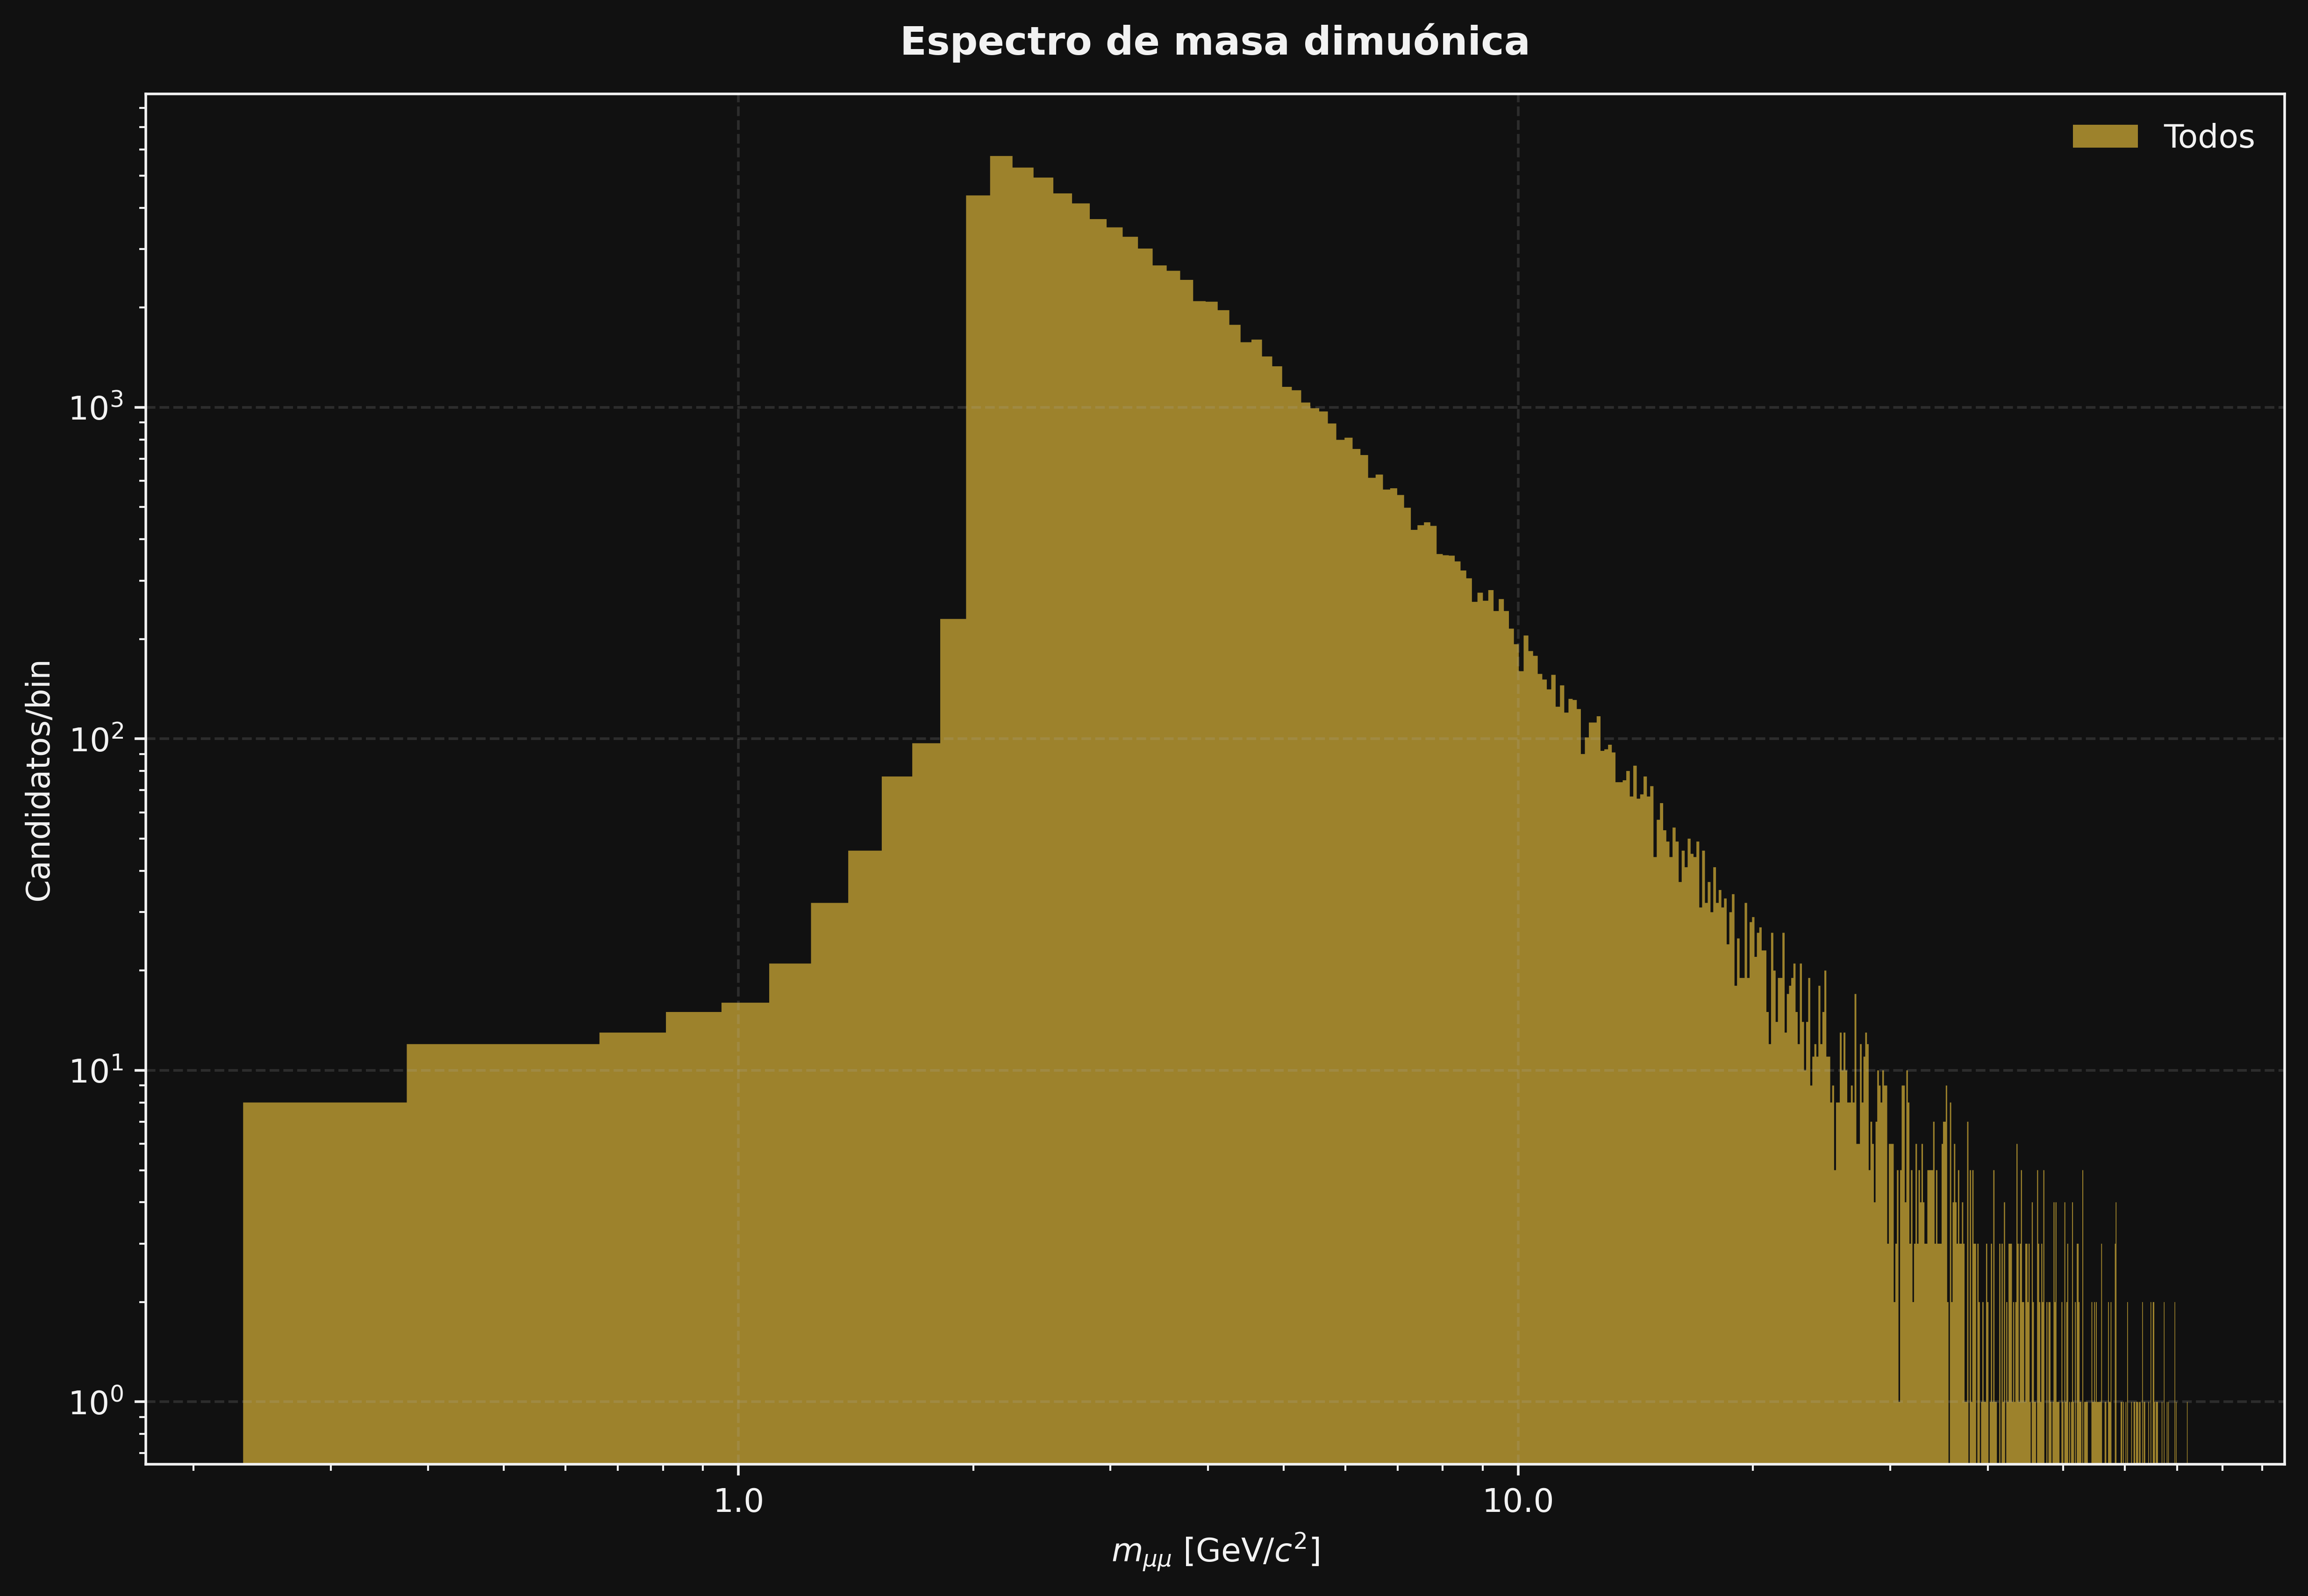
\includegraphics[width=\linewidth]{../assets/images/delphes/sm_model/c01/dimuon_mass_70GeV_01.png} } & { \textit{X: esc. log. \& Y: esc. log. (sin corte) - 70 $[GeV]$}\\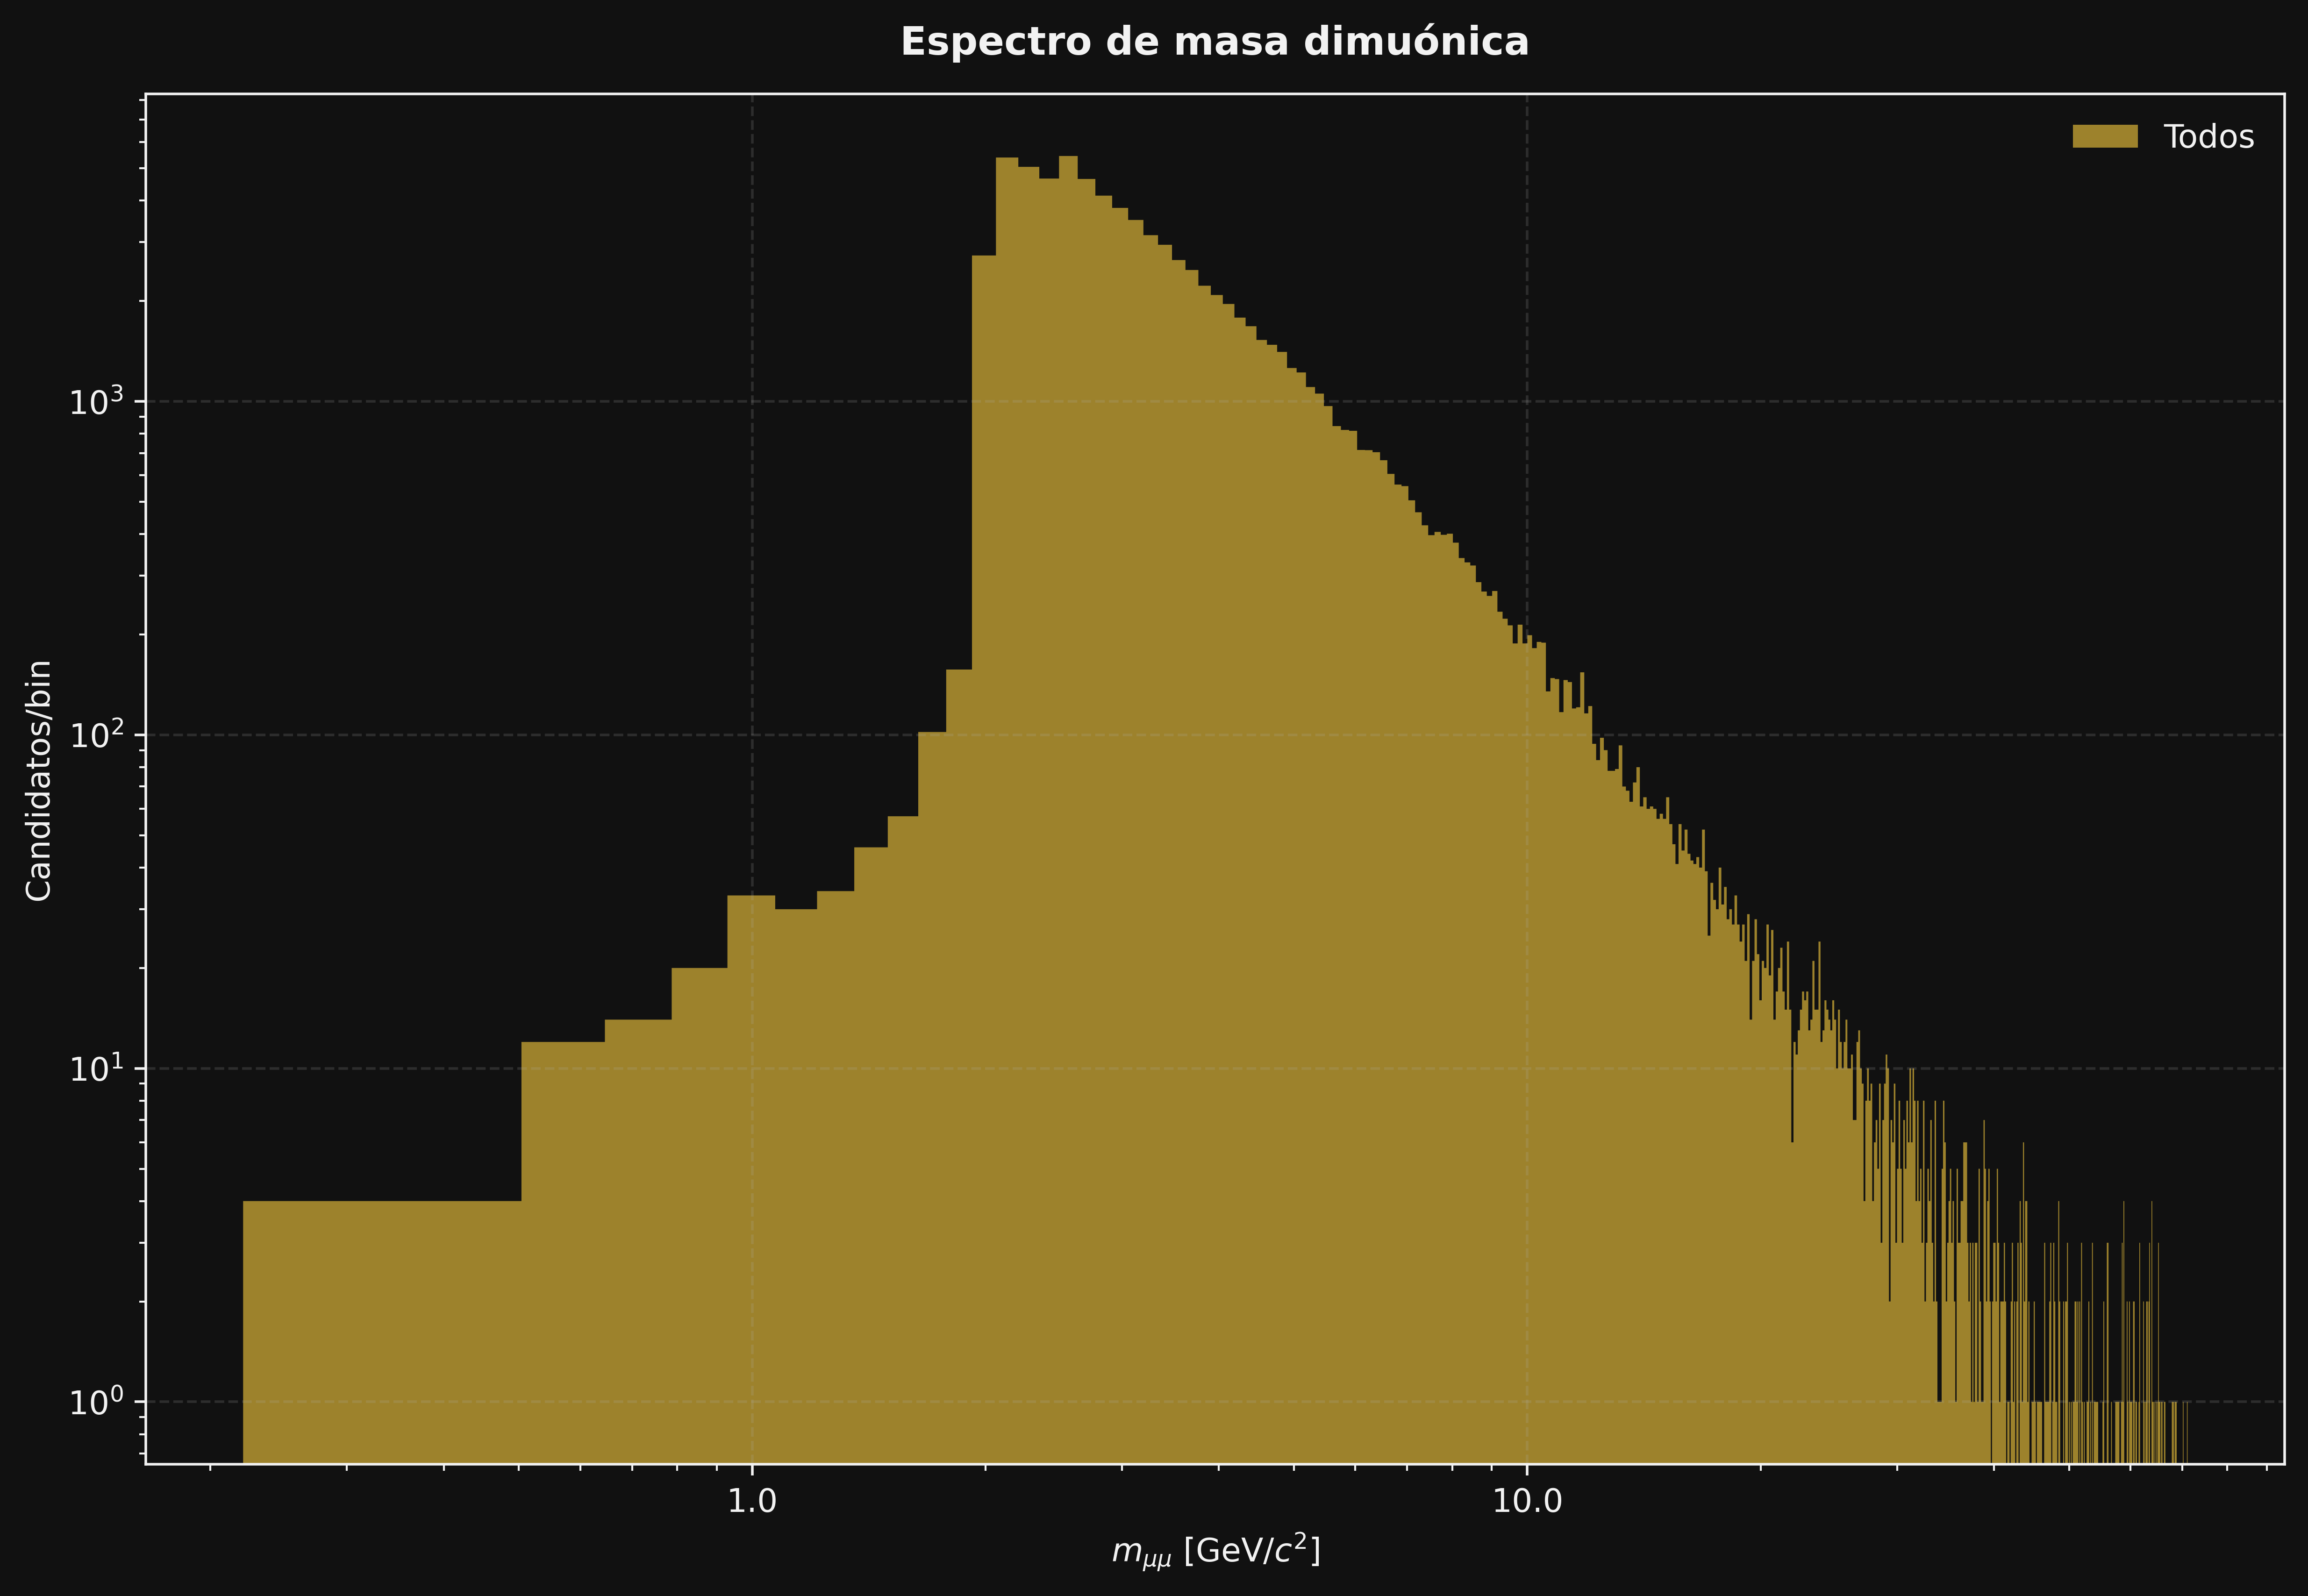
\includegraphics[width=\linewidth]{../assets/images/delphes/smf_model/c01/dimuon_mass_70GeV_01.png} } \\
    { \textit{X: esc. log. \& Y: esc. log. (corte) - 70 $[GeV]$}\\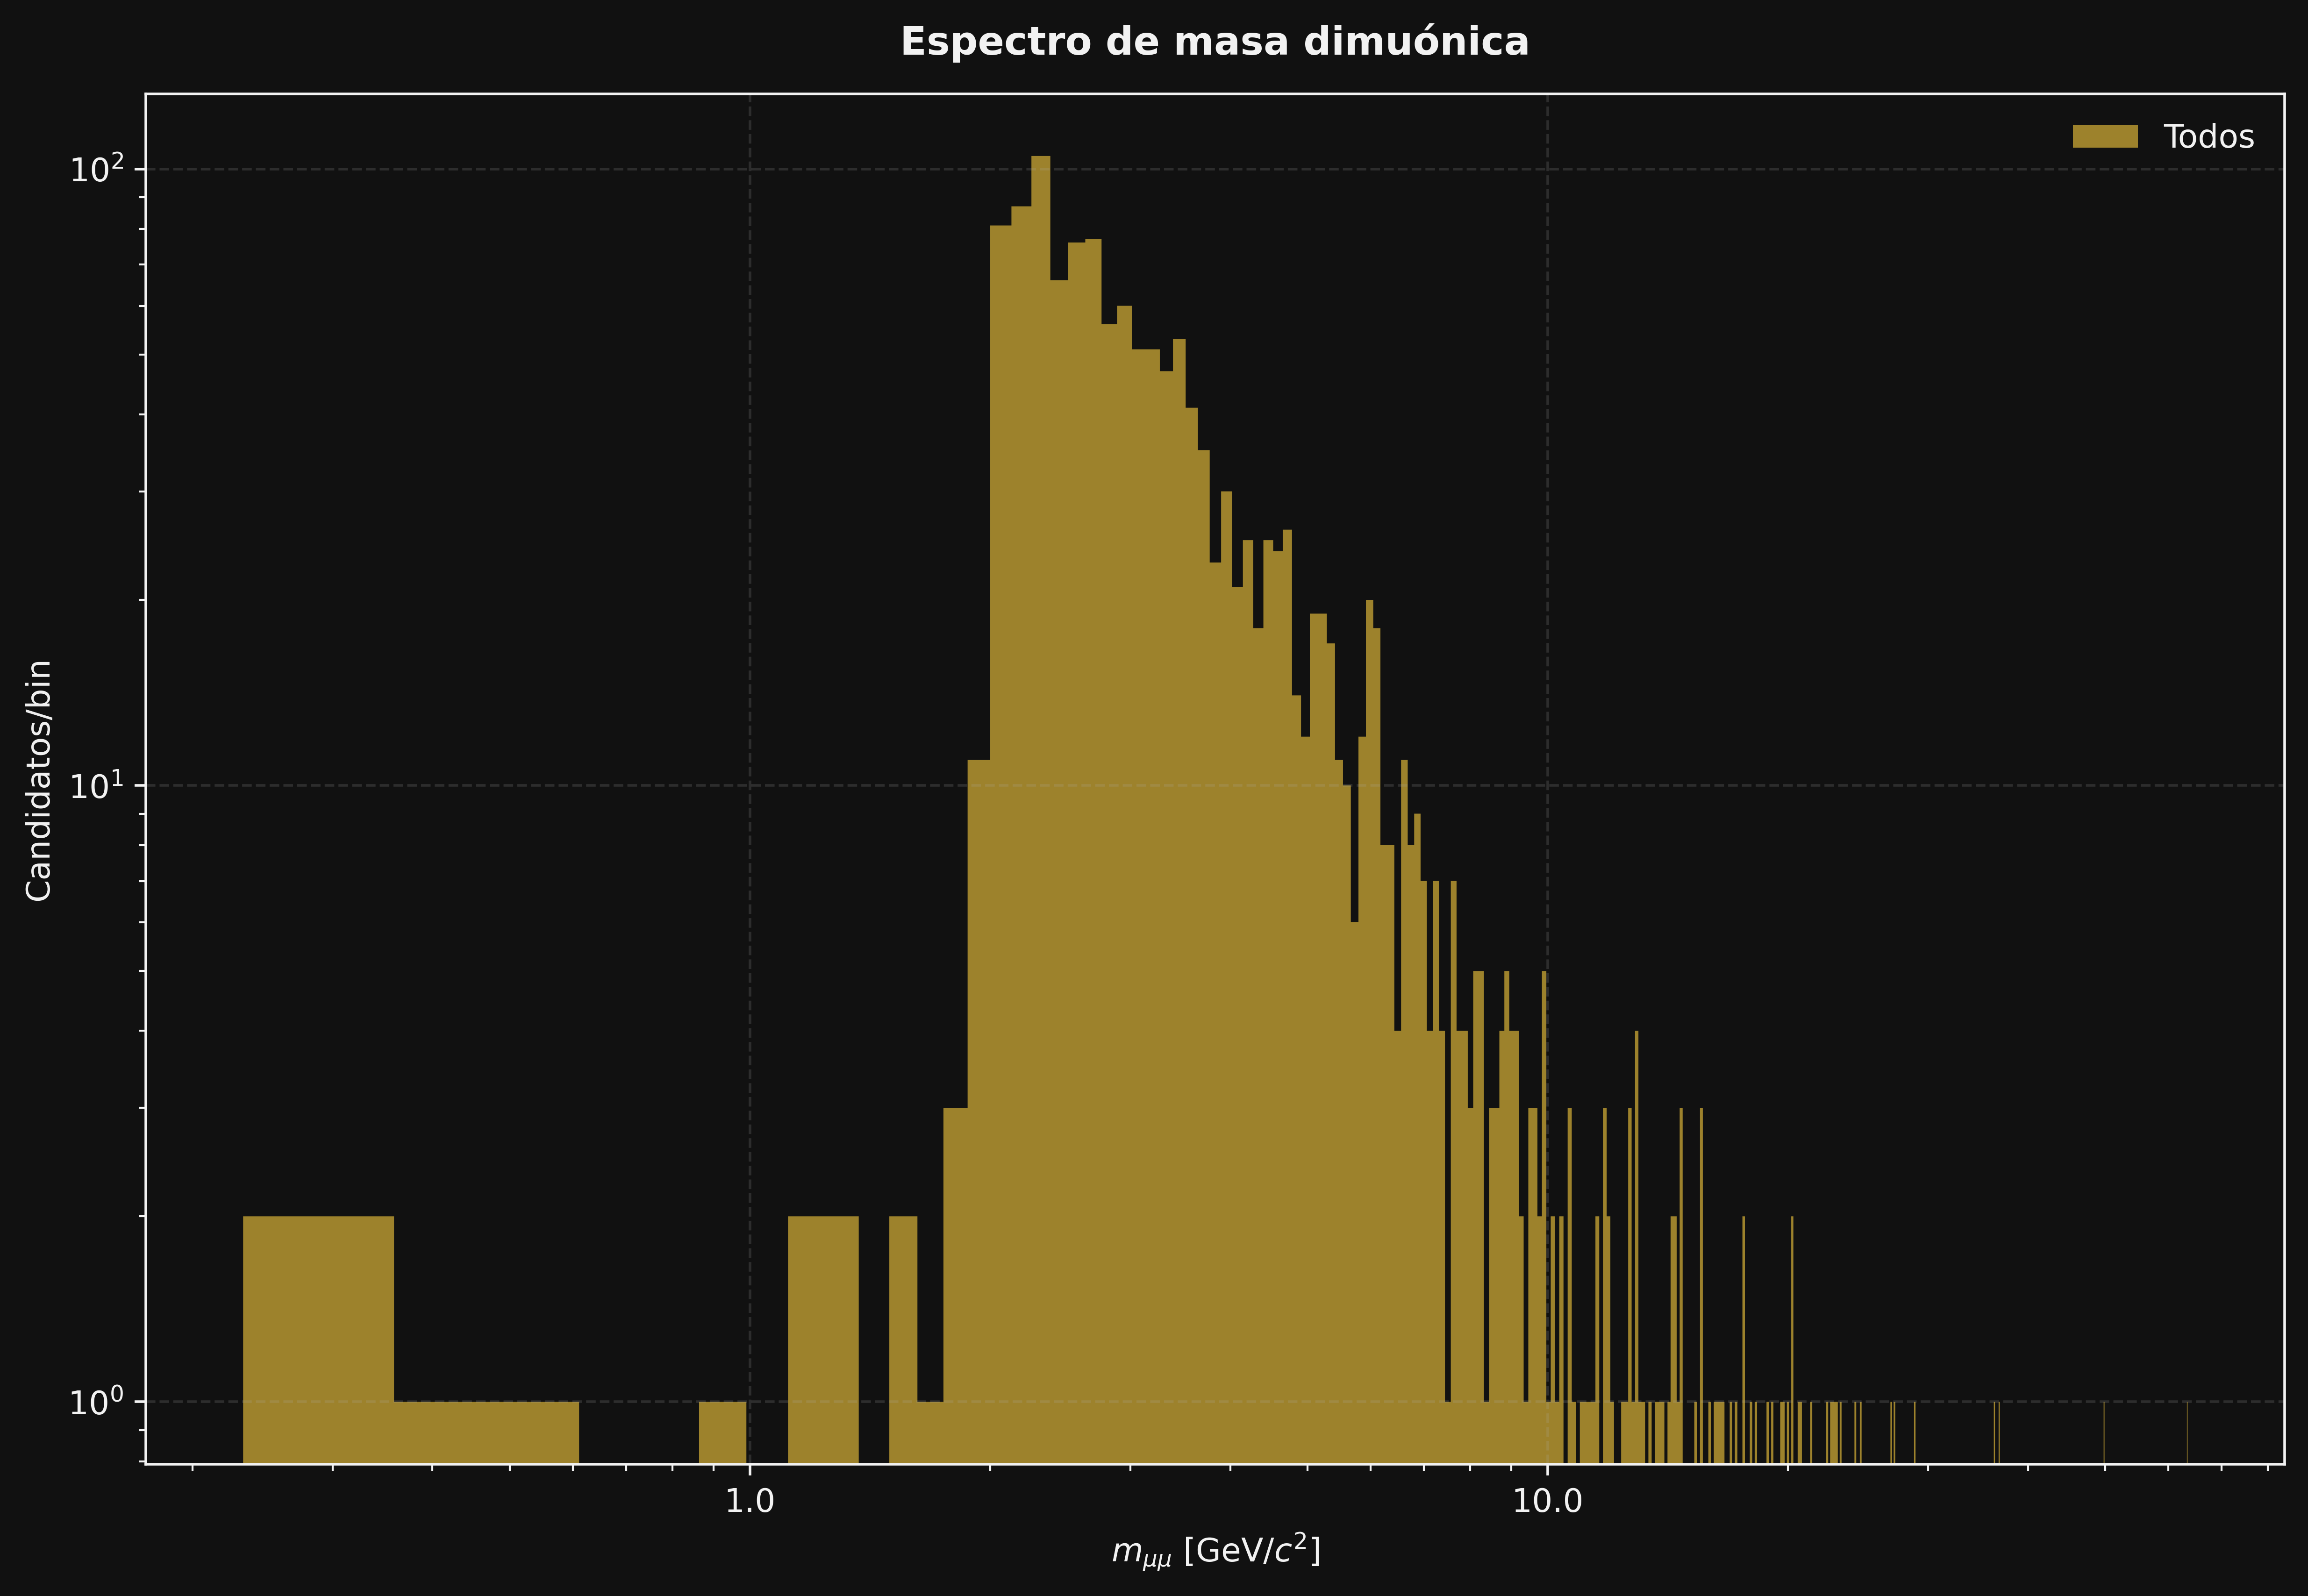
\includegraphics[width=\linewidth]{../assets/images/delphes/sm_model/c01/dimuon_mass_70GeV_01_cut.png} } & { \textit{X: esc. log. \& Y: esc. log. (corte) - 70 $[GeV]$}\\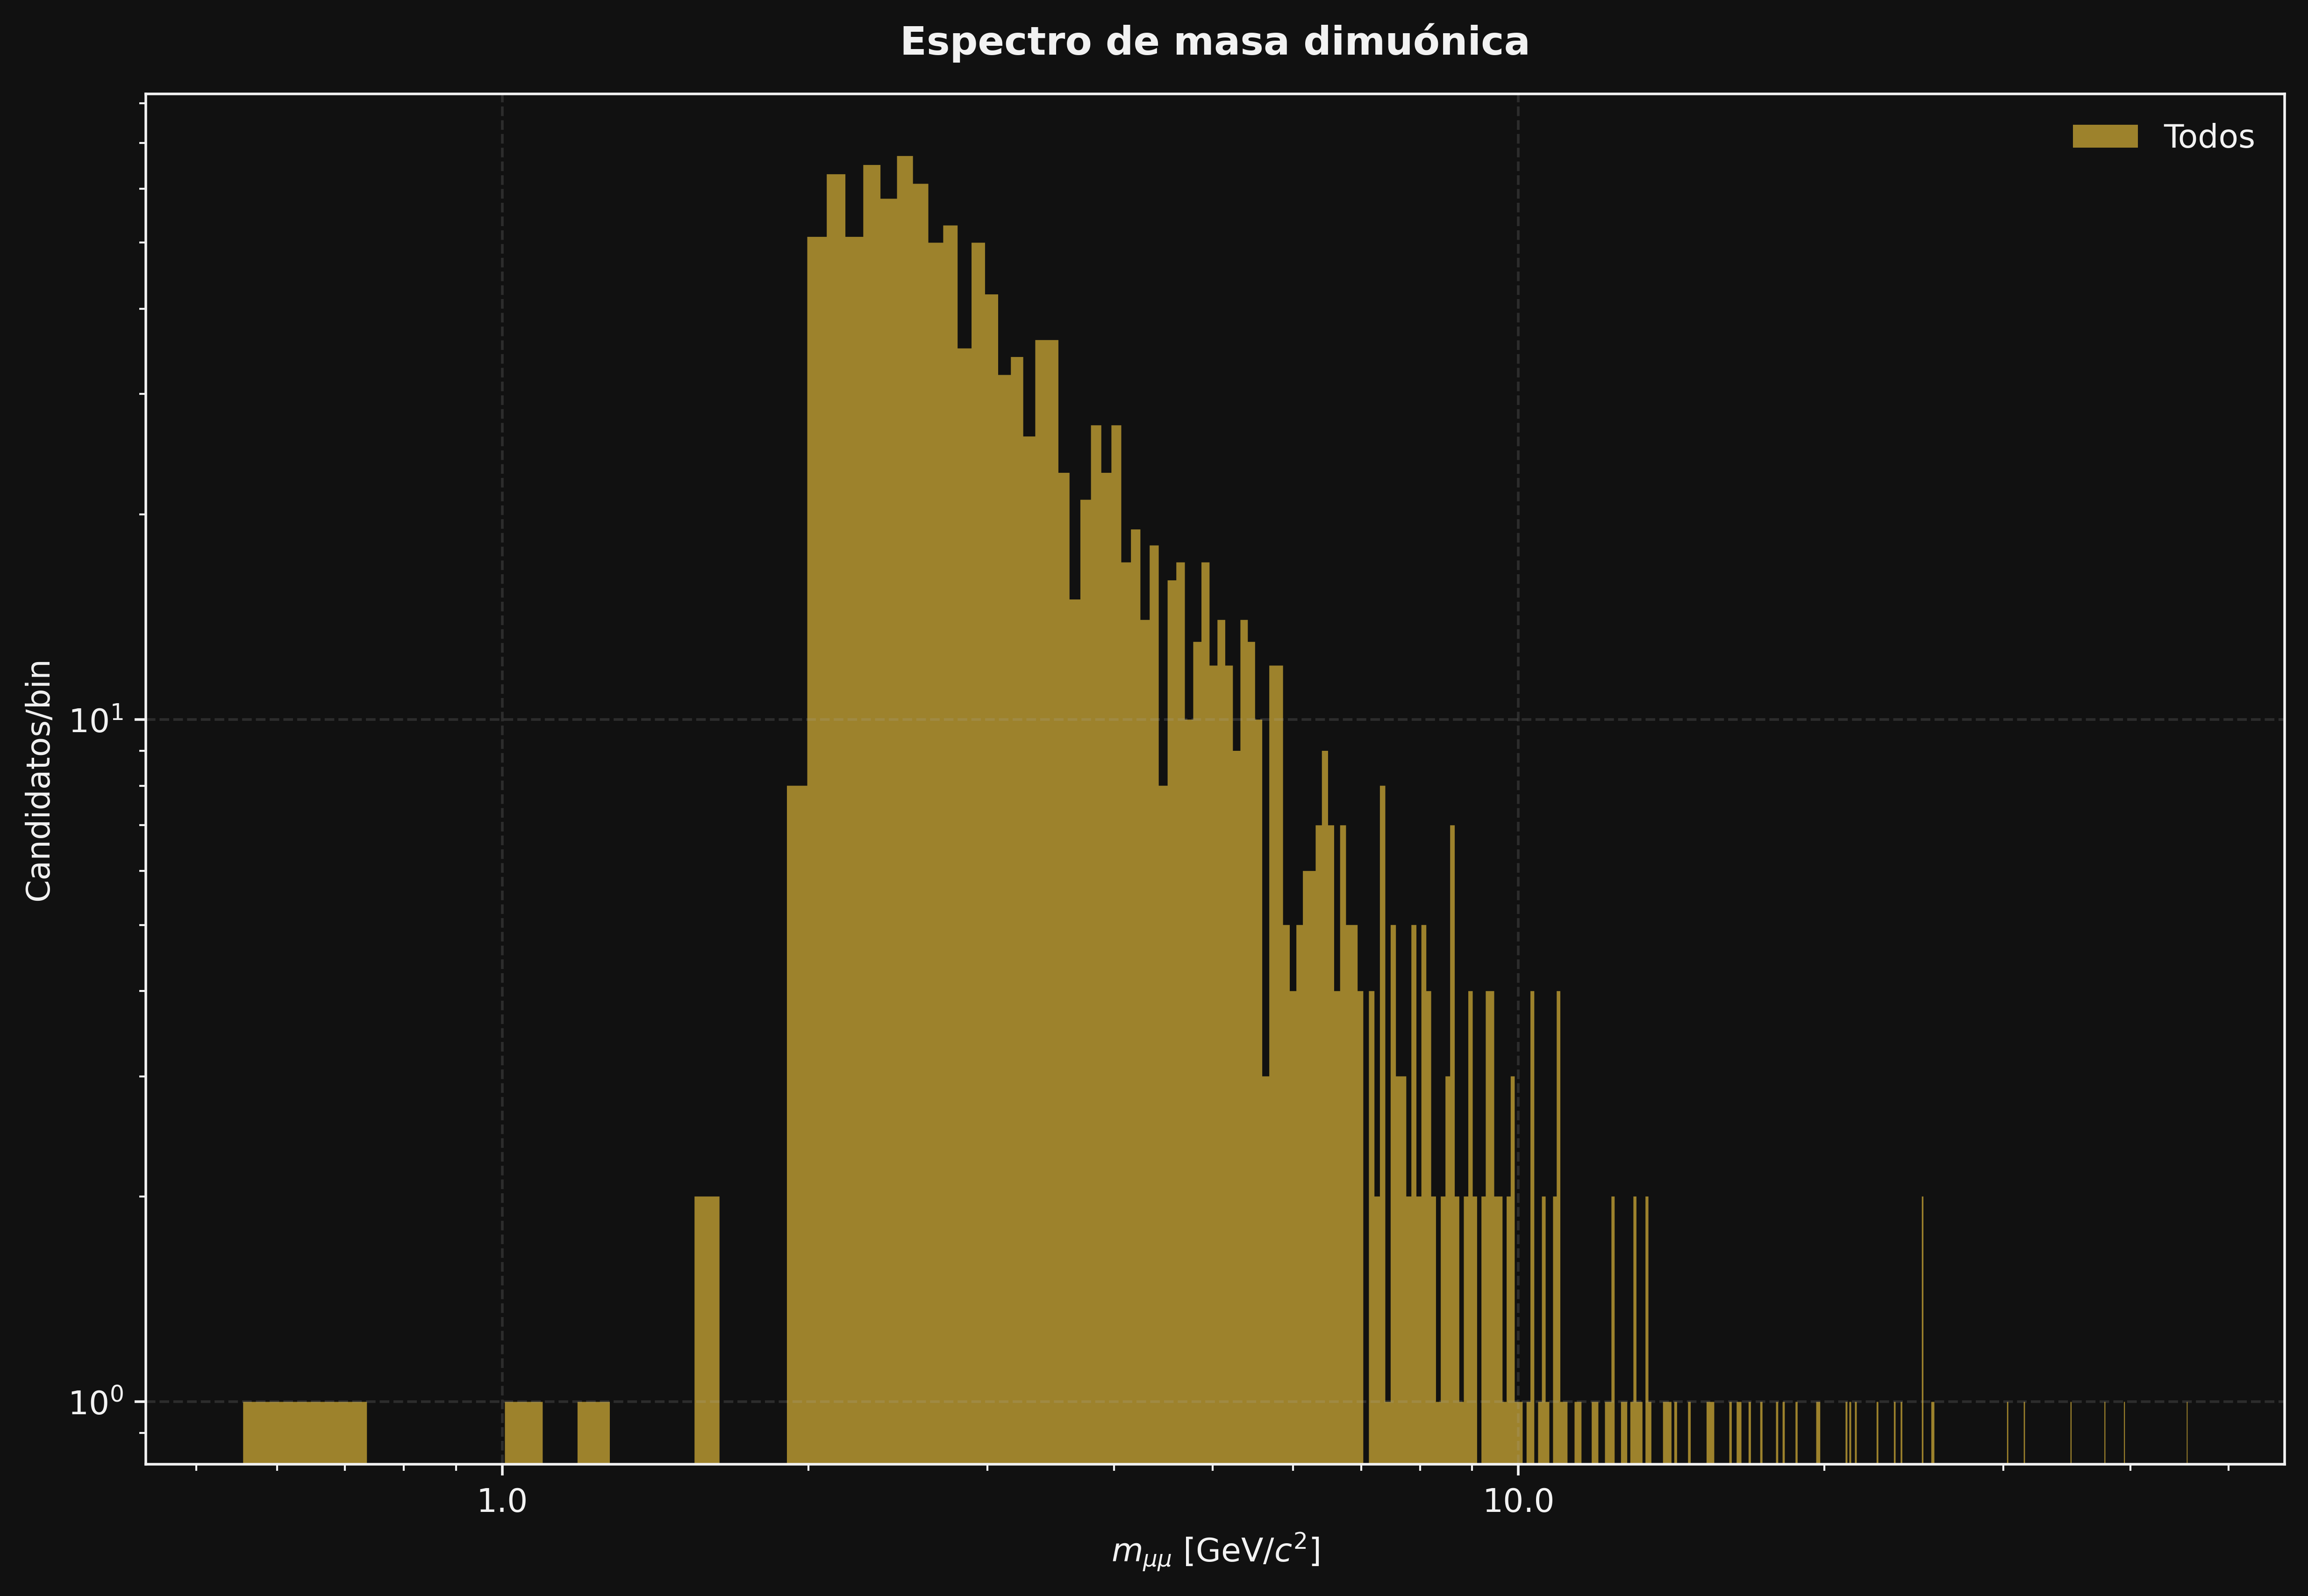
\includegraphics[width=\linewidth]{../assets/images/delphes/smf_model/c01/dimuon_mass_70GeV_01_cut.png} } \\\hline\hline
    \SetCell[c=2]{j}{\textbf{Observación: Prueba 03}} \\
    {Se aplicaron aceptaciones del LHCb según la tarjeta delphes\_card\_LHCb.tcl dentro de delphes\_card.dat. La formula de eficiencia para el módulo MuonTrackingEfficiency es una aproximación considerada de la literatura leida en el documento \textit{Measurement of the track reconstruction efficiency at LHCb} para trazas largas, dado que no se encontro más documentación del tracking de Muones en el LHCb.} & {Las gráficas estan realizadas con una escala logarítmica en el eje y, mientras que se le aplica la escala logarítmica a la masa invariante para graficarla directamente en el eje x sin tener que aplicar escala logarítmica en el eje, para evitar perder la visibilidad de los bines ubicados en la región de $m_{\mu\mu}>10.0\,[GeV]$.} \\
    \textbf{Modelo sm} & \textbf{Modelo sm-full} \\
    { \textbf{x: esc. lineal \& y: esc. log.}\\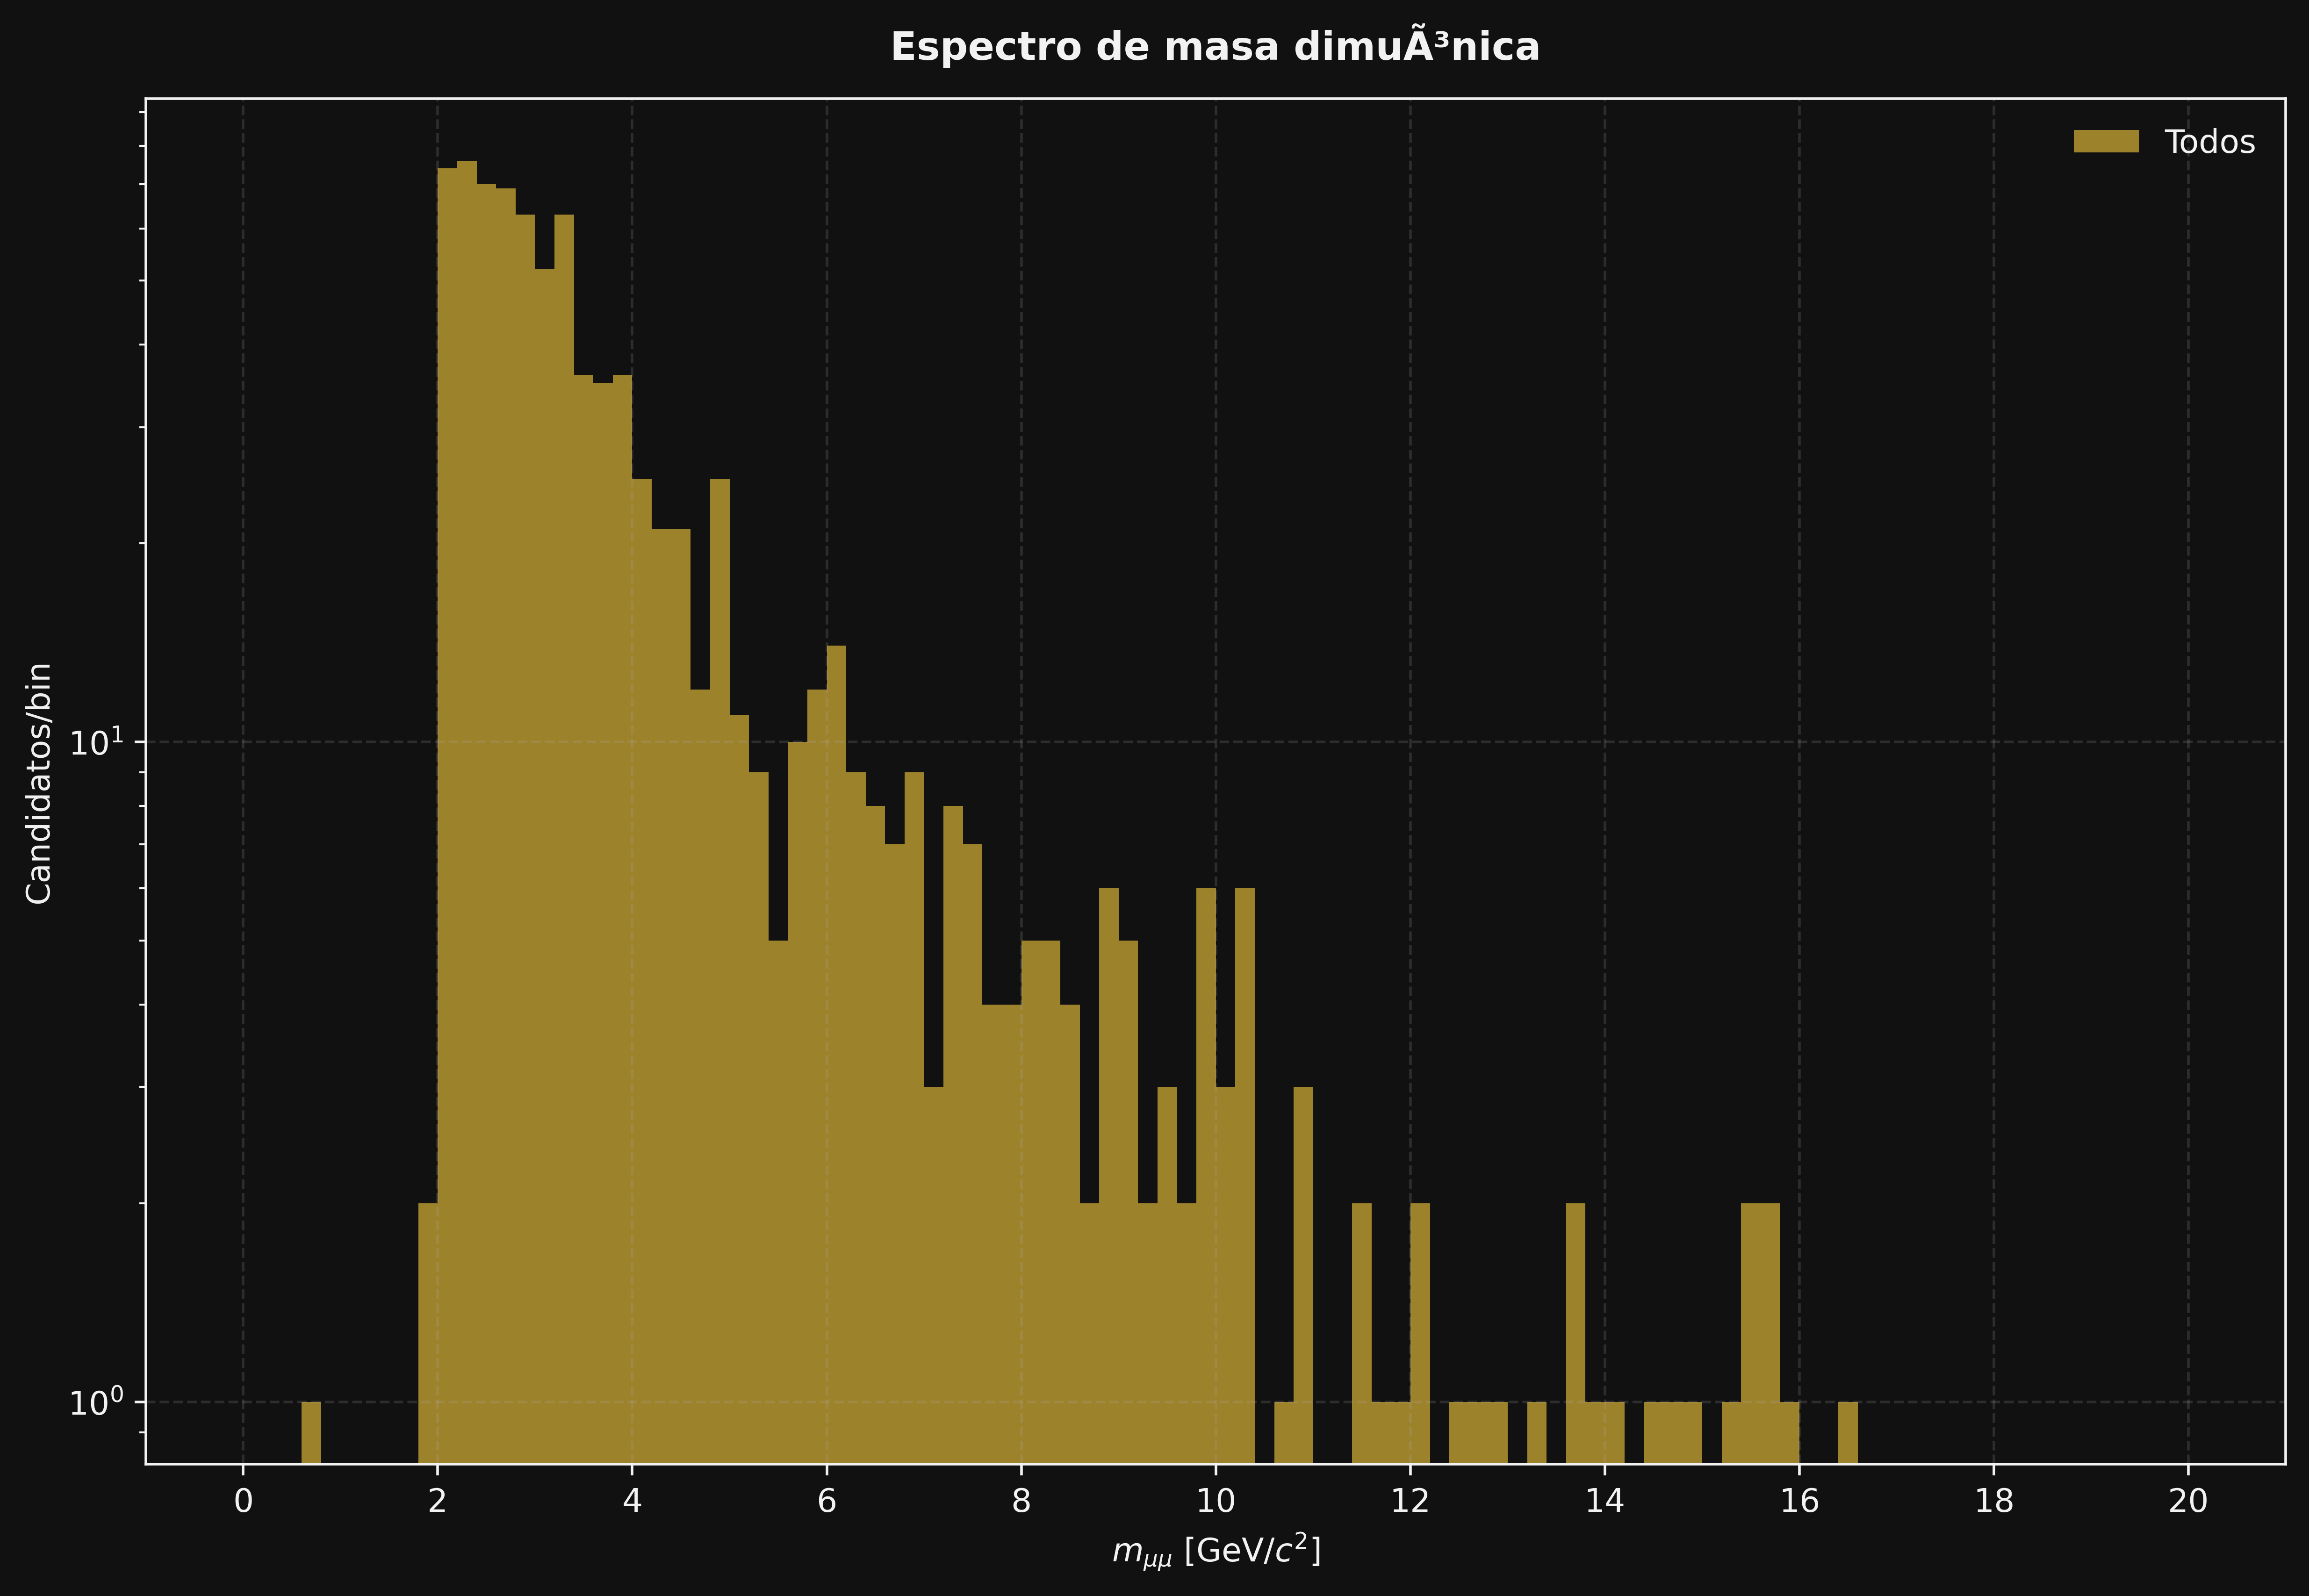
\includegraphics[width=\linewidth]{../assets/images/delphes/sm_model/c02/dimuon_mass_70GeV_00.png} } & { \textbf{x: esc. lineal \& y: esc. log.}\\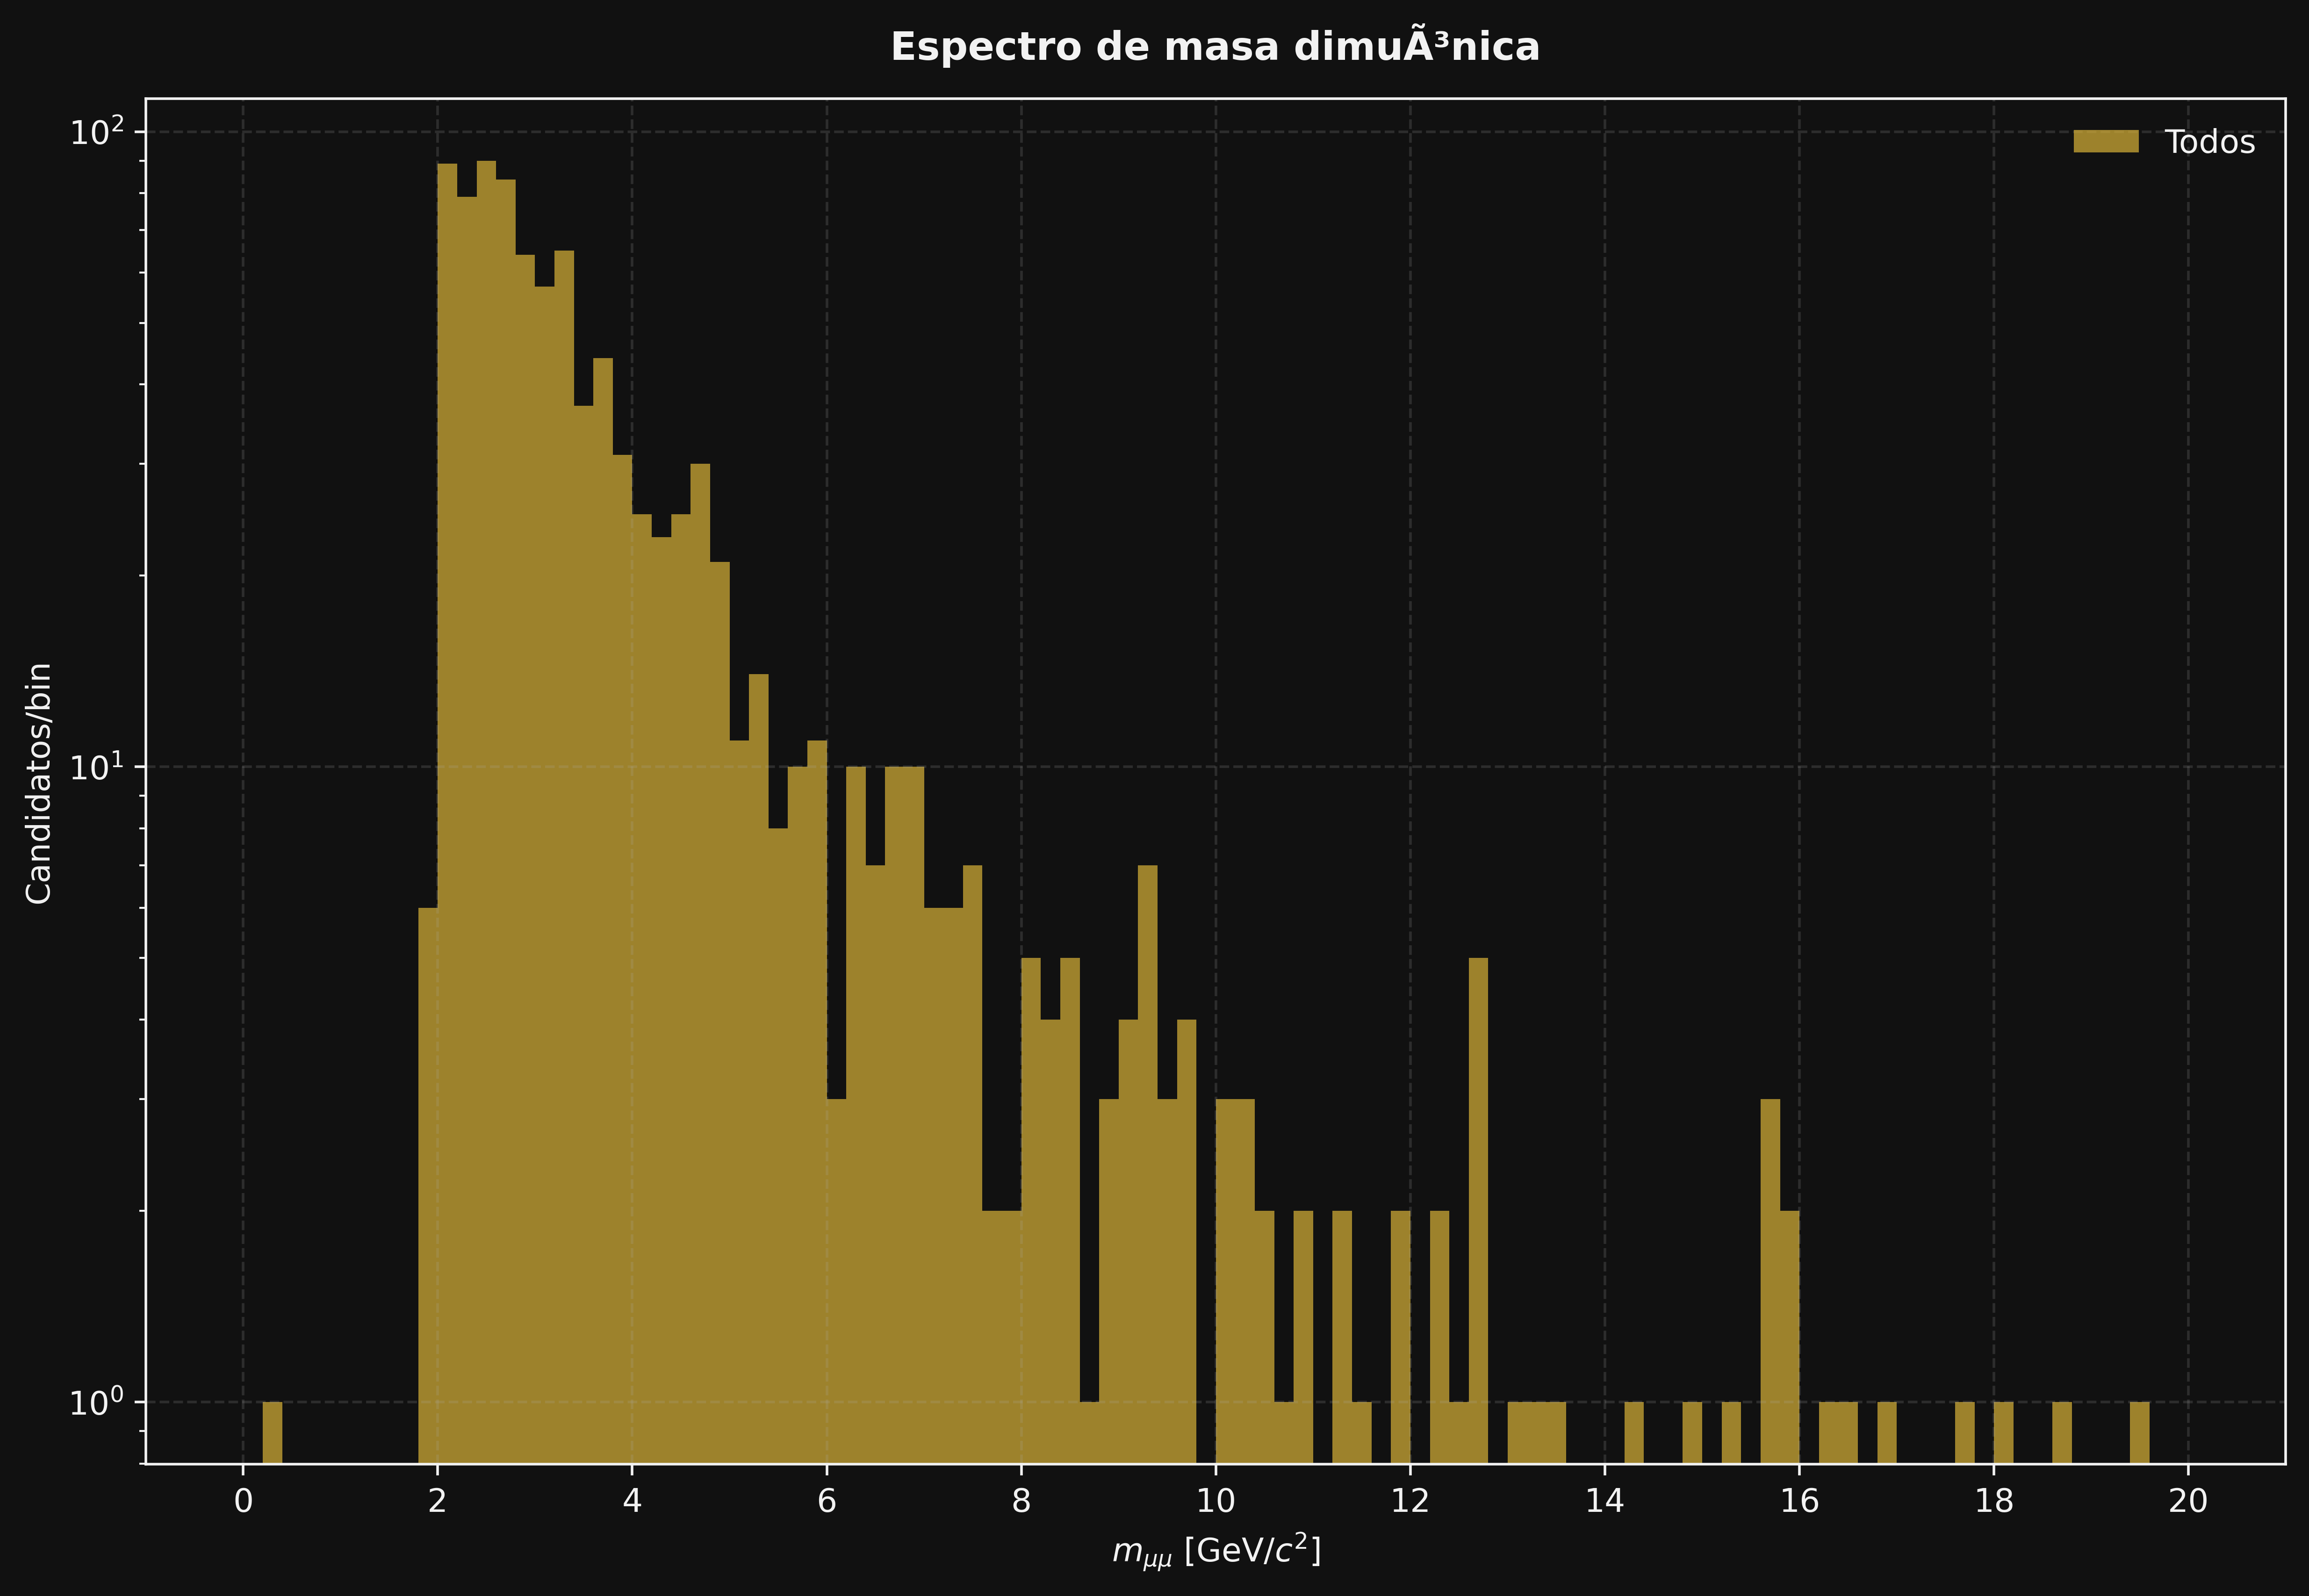
\includegraphics[width=\linewidth]{../assets/images/delphes/smf_model/c02/dimuon_mass_70GeV_00.png} } \\
    { \textbf{x: esc. log. \& y: esc. log.}\\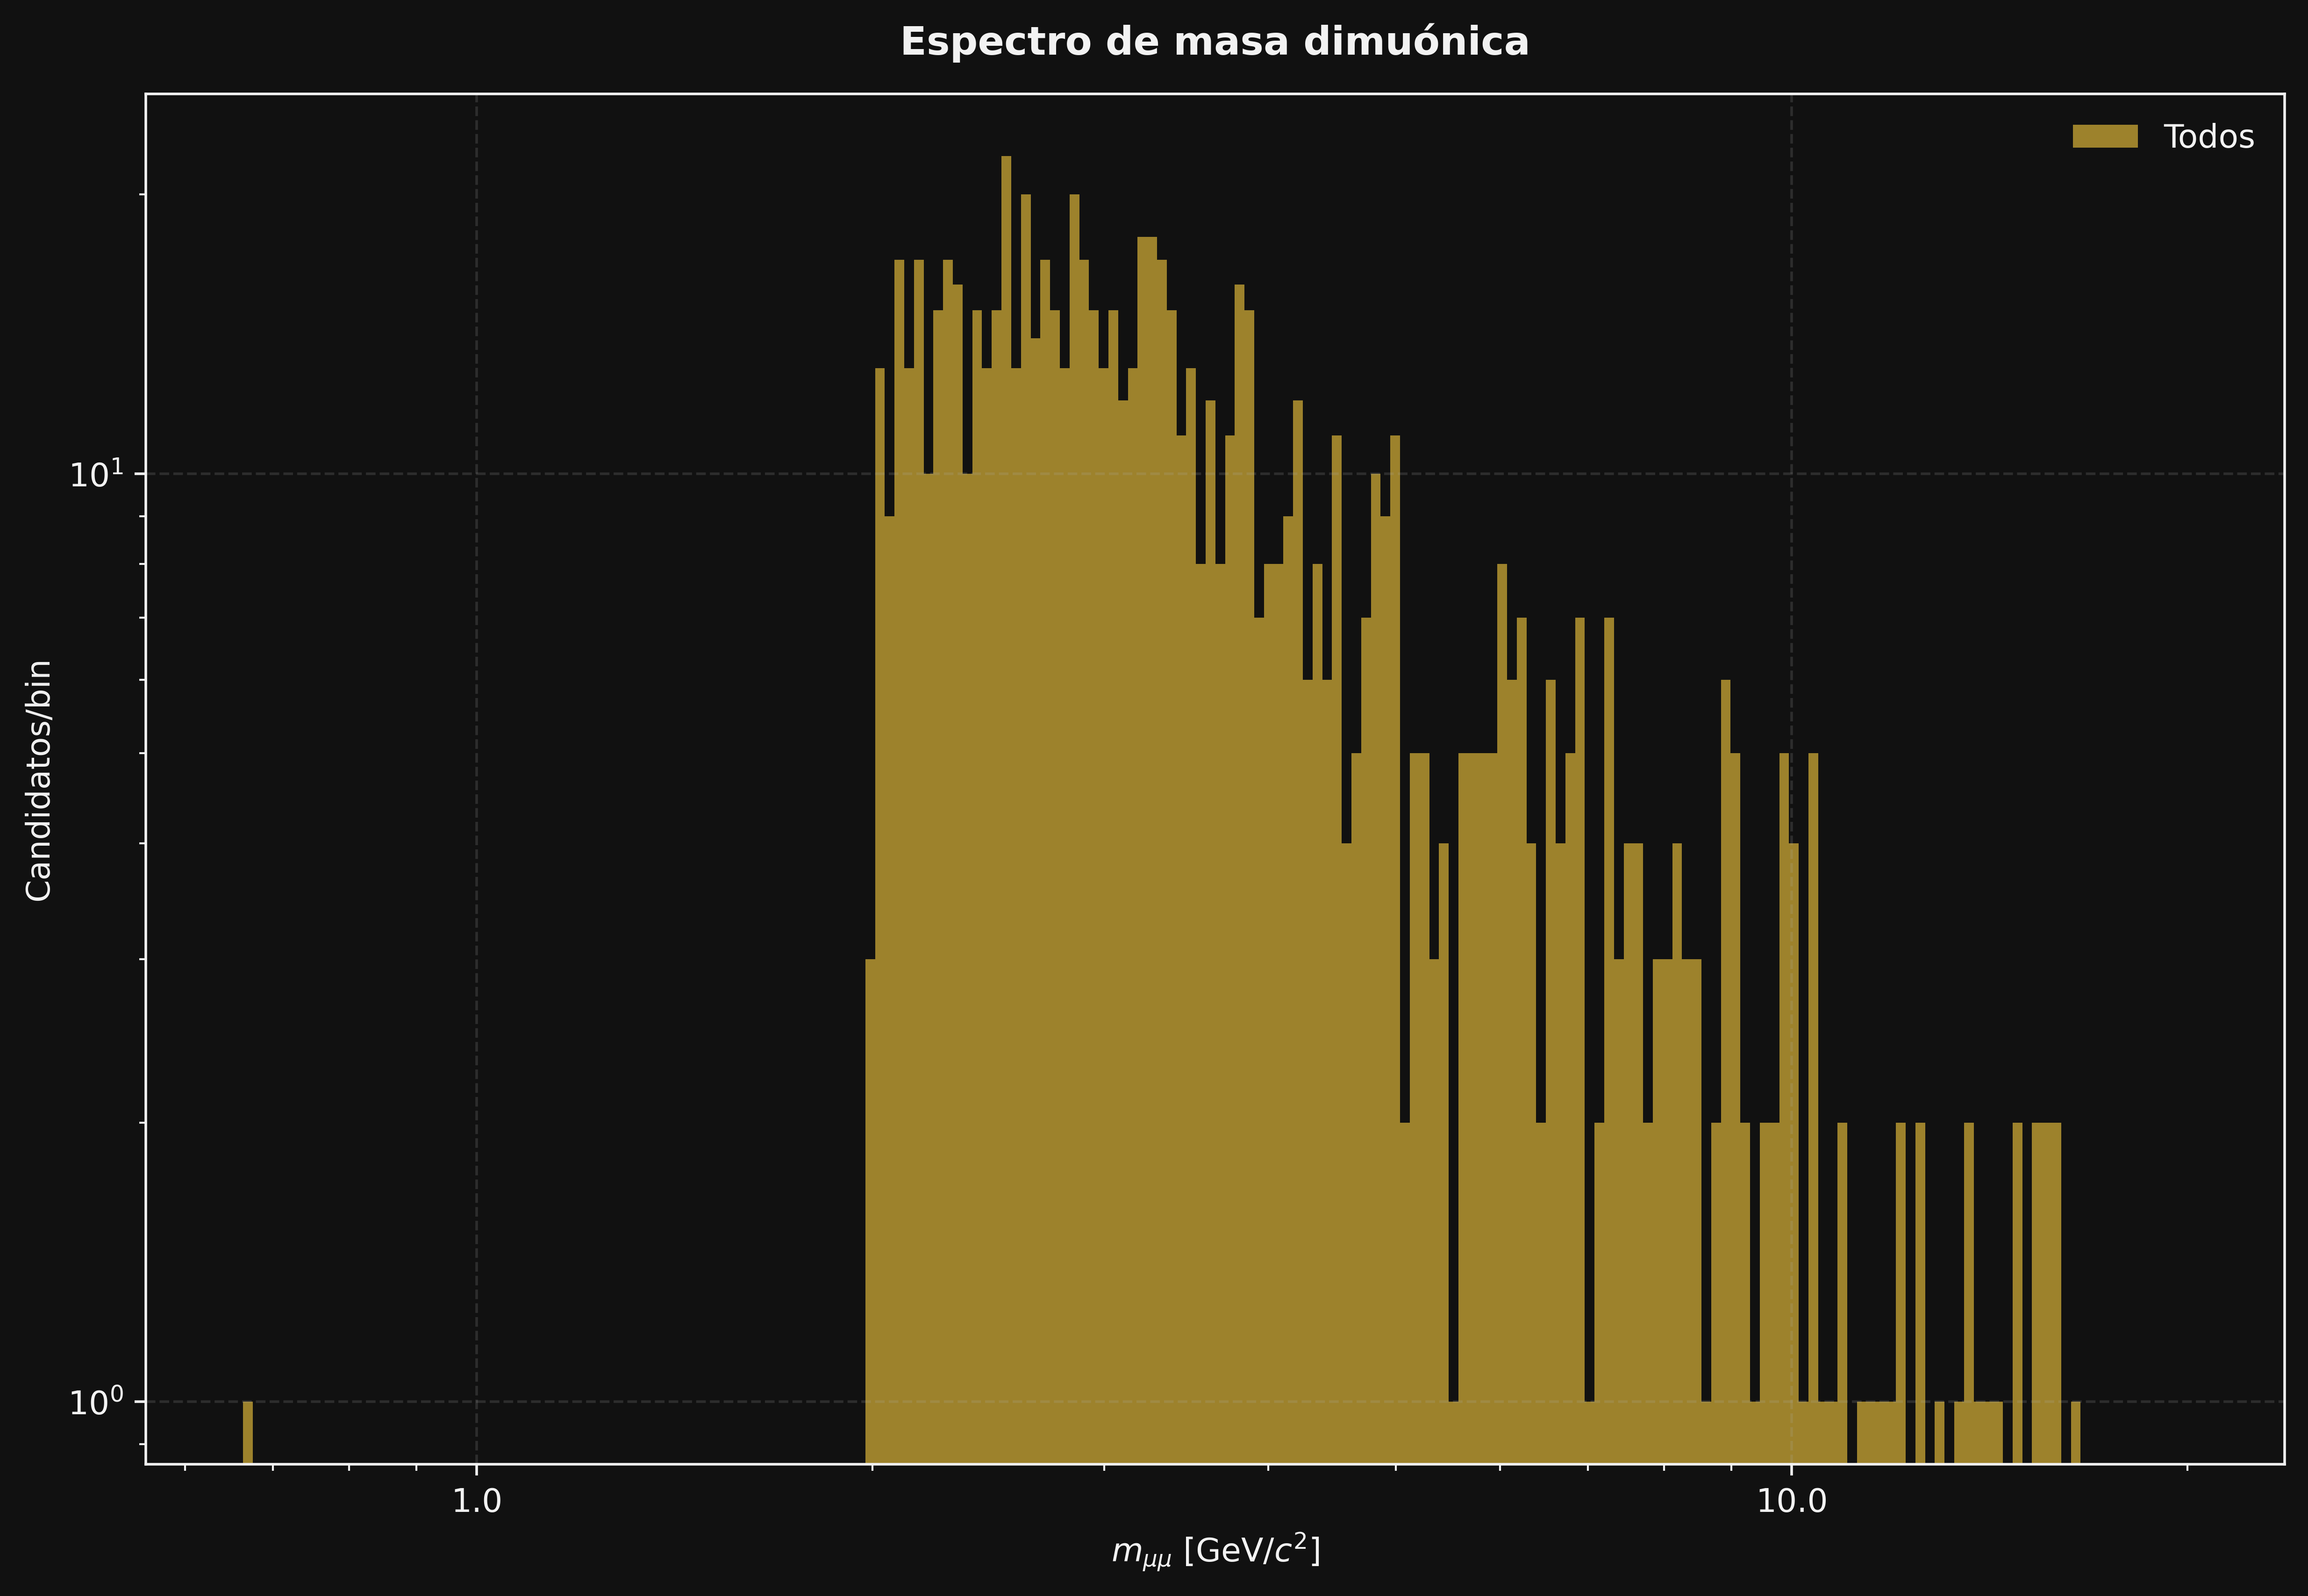
\includegraphics[width=\linewidth]{../assets/images/delphes/sm_model/c02/dimuon_mass_70GeV_01.png} } & { \textbf{x: esc. log. \& y: esc. log.}\\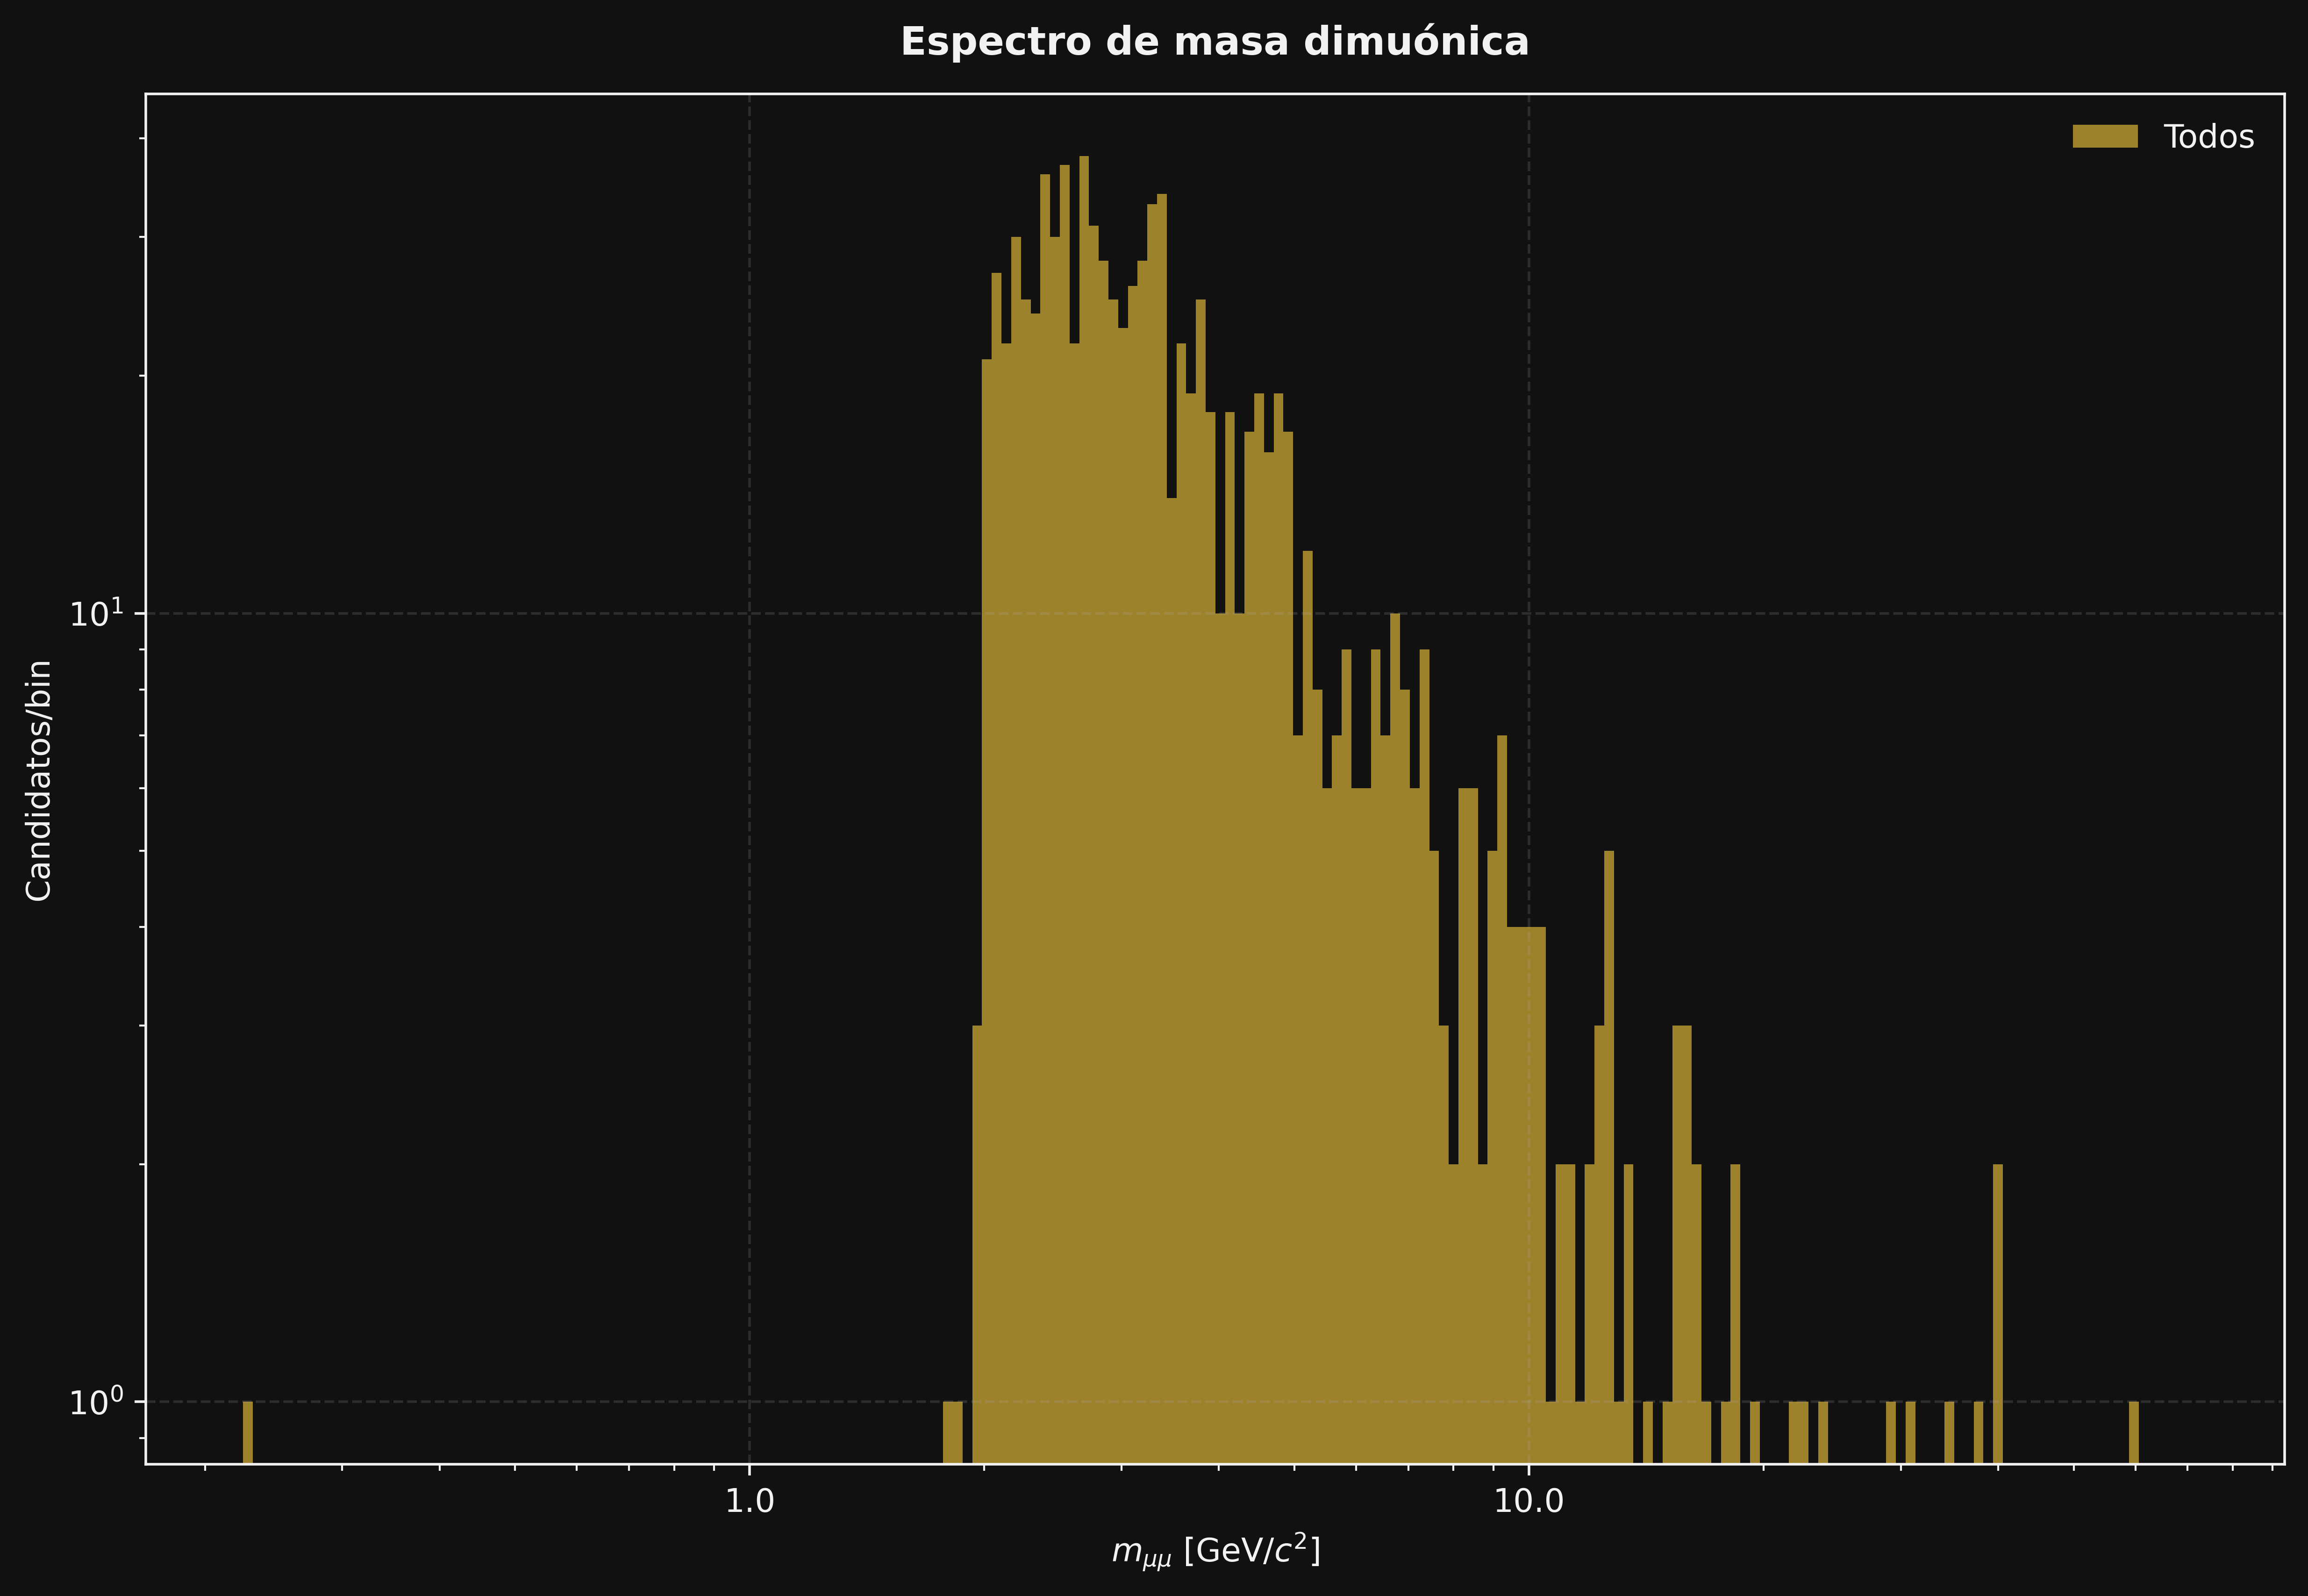
\includegraphics[width=\linewidth]{../assets/images/delphes/smf_model/c02/dimuon_mass_70GeV_01.png} } \\
\end{longtblr}